\documentclass[12pt,a4paper,oneside]{report}
\usepackage[utf8]{inputenc}
\usepackage[T1]{fontenc}
\usepackage{amsmath}
\usepackage{amsfonts}
\usepackage{amssymb}
\usepackage{graphicx}
\usepackage{fontspec}
\usepackage{titlesec}
\usepackage{tocloft}
\usepackage[margin=2.5cm]{geometry}
\usepackage{lipsum}
\usepackage[skip=10pt]{parskip}
\usepackage{mwe,tikz}
\usepackage{tabto}
\usepackage{dashrule}
\usepackage[backend=biber,style=authoryear]{biblatex}
\usepackage{listings,lstautogobble}
\usepackage{scrextend}
\usepackage{enumitem}
\usepackage{hyperref}
\usepackage{float}
\usepackage{wrapfig}

\ifdefined\EasyMarkPrivateBuild
	\input{private.tex}
	\newcommand{\IfPrivateBuild}[2]{#1}
\else
	\newcommand{\IfPrivateBuild}[2]{#2}
\fi

\addbibresource{citations.bib}

\setcounter{secnumdepth}{3}
\addtolength{\textwidth}{-1cm}
\addtolength{\oddsidemargin}{1cm}
\addtolength{\evensidemargin}{1cm}

\lstset{autogobble=true}
\lstset{language=sh,basicstyle=\ttfamily}
\lstset{language=java,basicstyle=\ttfamily}

% Calibri or sans-serif as default font
\defaultfontfeatures{Mapping=tex-text,Scale=MatchLowercase}
\IfFontExistsTF{Calibre}{
	\setmainfont{Calibre}
}{
	\renewcommand{\familydefault}{\sfdefault}
}

% TOC horizontal spacing
\cftsetindents{chapter}{0cm}{1cm}
\cftsetindents{section}{1cm}{1cm}
\cftsetindents{subsection}{2cm}{1.2cm}

% TOC vertical spacing
\renewcommand{\cftchapfont}{
	\bfseries
	\fontsize{13pt}{13pt}
	\selectfont
	\vspace{6pt}
}
\cftbeforechapskip12pt
\renewcommand{\cftsecfont}{
	\fontsize{11pt}{11pt}
	\selectfont
	\vspace{6pt}
}
\cftbeforesecskip6pt
\renewcommand{\cftsubsecfont}{
	\fontsize{10pt}{10pt}
	\selectfont
	\vspace{3pt}
}
\cftbeforesubsecskip6pt

% TOC title
\renewcommand\cfttoctitlefont{
	\hfill
	\fontsize{16pt}{16pt}
	\selectfont
	\bfseries
}
\cftbeforetoctitleskip6pt
\cftaftertoctitleskip12pt

% Title format for chapter, section, sub- and subsubsection
% See https://tex.stackexchange.com/questions/511981/titlesec-vertical-align-chapter-and-section
% The -5pt is just pixel pushing bc I couldn't figure out why my chapter/section/subsection/subsubsection headings are slightly indented
\titleformat{\chapter}[hang]{
	\normalfont
	\bfseries
	\filright
	\fontsize{16pt}{16pt}
	\selectfont
}{
	\makebox[1.7cm][l]{\thechapter}
}{0em}{}
\titlespacing{\chapter}{-5pt}{18pt}{12pt}

\titleformat{\section}[hang]{
	\normalfont
	\bfseries
	\filright
	\fontsize{14pt}{14pt}
	\selectfont
}{
	\makebox[1.7cm][l]{\thesection}
}{0em}{}
\titlespacing{\section}{-5pt}{18pt}{12pt}

\titleformat{\subsection}[hang]{
	\normalfont
	\bfseries
	\filright
	\fontsize{12pt}{12pt}
	\selectfont
}{
	\makebox[1.7cm][l]{\thesubsection}
}{0em}{}
\titlespacing{\subsection}{-5pt}{18pt}{12pt}

\titleformat{\subsubsection}[hang]{
	\normalfont
	\bfseries
	\filright
	\fontsize{11pt}{11pt}
	\selectfont
}{
	\makebox[1.7cm][l]{\thesubsubsection}
}{0em}{}
\titlespacing{\subsubsection}{-5pt}{12pt}{12pt}

\newcommand{\IncludeSchoolTemplate}[2]{
	\vspace*{-7em}
	\makebox[\textwidth]{
		\begin{tikzpicture}[
			every node/.style={anchor=north west,inner sep=0pt},
			x=1mm, y=1mm]
			\node (templatepage) at (0,0)
				{\includegraphics[width=\paperwidth,page=#1]{summary.pdf}};
			#2
		\end{tikzpicture}
	}
	\newpage
}

\newcommand{\SignatureLine}[1]{
	\vskip15pt
	\tabto{9cm}#1
	\vskip10pt
	\tabto{9cm}\hdashrule[0pt][x]{\fill}{.5pt}{.75mm}
}

\newcommand{\BlockCite}[2]{
	\begin{addmargin}[1cm]{0pt}
		#1

		\fullcite{#2}
	\end{addmargin}
}

\newcounter{appendix}
\newcommand{\Appendix}[1]{
	\stepcounter{appendix}
	\chapter*{\hspace{\fill}Appendix \Alph{appendix}} \label{app:\Alph{appendix}}
	#1
}

\newcommand{\RefAppendix}[1]{\hyperref[app:#1]{Appendix~#1}}


\title{Easy Mark One}
\author{\IfPrivateBuild{\EmRealAuthorName}{T0astBread}}

\begin{document}
	\pagenumbering{gobble}
	\maketitle
	\IfPrivateBuild{
		\chapter*{Erklärung gemäß Prüfungsordnung}
		„Ich erkläre an Eides statt, dass ich die vorliegende Diplomarbeit selbstständig und ohne fremde Hilfe verfasst, andere als die angegebenen Quellen und Hilfsmittel nicht benutzt und alle den benutzten Quellen wörtlich oder sinngemäß entnommenen Stellen als solche kenntlich gemacht habe.“

		\EmPhysicalLocation, \today\tabto{9cm}{Verfasser*innen:}

		\SignatureLine{\EmRealAuthorName}
		\newpage
		\IncludeSchoolTemplate{1}{
			\node at (77,-28)
				{Informatik};
			\node at (77,-63)
				{\EmRealAuthorName};
			\node at (77,-80)
				{2019/20};
			\node at (77,-92)
				{Easy Mark One};
			\node at (77,-109)
				{\EmPartner};
			\node at (77,-127) [text width=305,align=justify] {
				\fontsize{12pt}{12pt}
				\selectfont
				\par
				Ziel des Projekts war die Entwicklung eines Tools zur Teilautomatisierung des Bewertungsprozesses für Programmier(haus)aufgaben in der Programmiersprache Java (Teilprojekt \emph{Automark}), sowie einer Web-Plattform für Lehrer und Schüler, um Informationen zu Aufgaben und Bewertungen zu teilen (Teilprojekt \emph{EasyMark}).
				\vskip10pt
				\par
				Alle Programme sollten in Java realisiert werden.
			};
			\node at (77,-174) [text width=300,align=justify] {
				\fontsize{12pt}{12pt}
				\selectfont
				\par
				Automark wurde als ein zusammenhängendes Java-Programm umgesetzt, das über die Kommandozeile sowie über eine GUI gesteuert werden kann. Diverse Libraries wurden für die zahlreichen Funktionen verwendet.
				\vskip10pt
				\par
				EasyMark wurde auf Basis des \emph{Javalin} Web-Frameworks entwickelt. Als Datenbank fungiert eine flache JSON-Datei mit Read/Write Lock. Für kryptographische Funktionen wurde Spring Security (als Standalone-Variante) verwendet.
			};
			\node at (77, -222) [text width=300,align=justify] {
				\fontsize{12pt}{12pt}
				\selectfont
				\par
				Automark: Die Teilaufgaben im Bewertungsprozess wurden zuerst implementiert, danach Nebenfunktionen wie Rollback/mark-resolved. Die GUI wurde entwickelt, um den Einstieg ins Programm zu erleichtern. Ebenfalls noch Zusatzfunktionen wie das automatische Versenden von Ergebnis-Emails und der Konfigurations-Wizard.
				\vskip10pt
				\par
				EasyMark: Zuerst wurden das Datenmodell und das Datenbanksystem entwickelt. Die Funktionalität würde zuerst abstrakt implementiert, dann die Business-Logic. Zuletzt wurde die Sicherheit des Servers überarbeitet und ein Programm zur Konfiguration eines Hosts geschrieben.
			};
		}
		\IncludeSchoolTemplate{2}{
			\node at (77,-28)
				{Informatik};
			\node at (77,-69){
				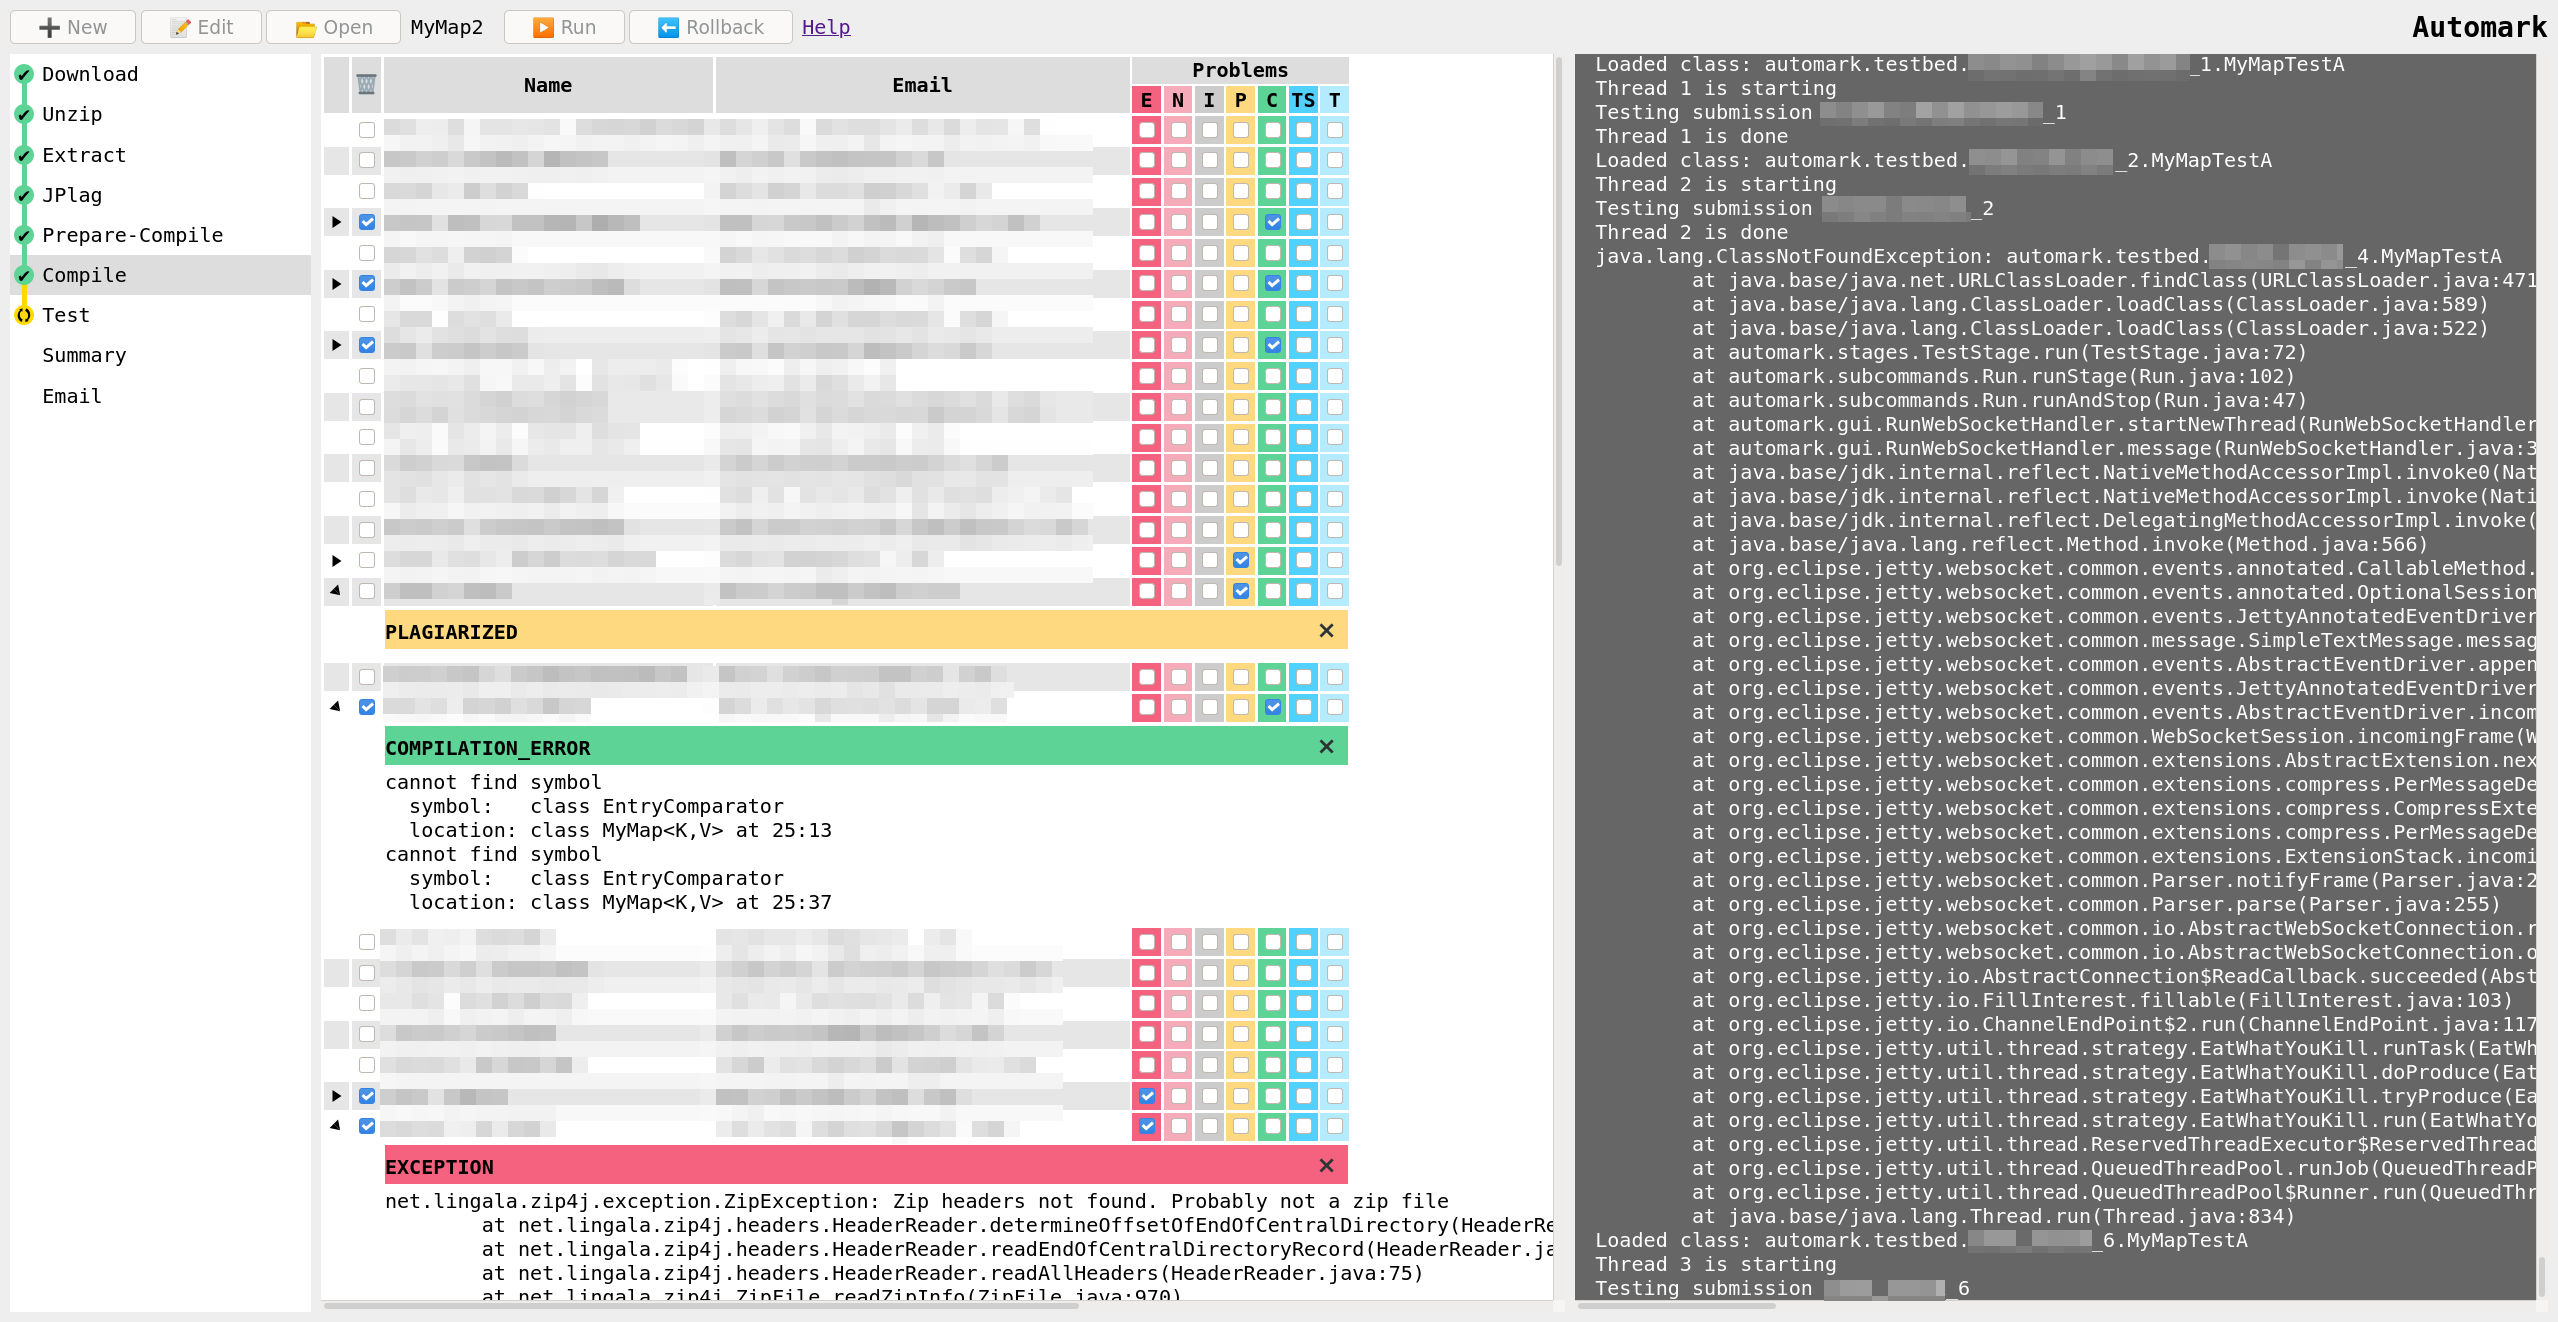
\includegraphics[width=310pt,trim=0pt 0pt 1110pt 0pt,clip]{automark_dashboard_w_details_expanded.png}
			};
			\node at (77,-171) [text width=305,align=center]
				{\emph{Screenshot der Automark-GUI (Ausschnitt). Links befindet sich eine Übersicht über alle Teilaufgaben im Prozess (\emph{Stages}), in der Mitte eine Tablle mit einer Übersicht sowie Details zu Schülerabgaben und deren Mängel. Persönlich identifizierbare Informationen sind unkenntlich gemacht.}};
			\node at (77,-220)
				{--};
			\node at (77,-239)
				{Öffentlich; Bibliothek der \EmSchoolName};
		}
		\IncludeSchoolTemplate{3}{
			\node at (76,-28)
				{Informatics};
			\node at (77,-63)
				{\EmRealAuthorName};
			\node at (77,-80)
				{2019/20};
			\node at (77,-92)
				{Easy Mark One};
			\node at (77,-109)
				{\EmPartner};
			\node at (77,-125) [text width=305,align=justify] {
				\fontsize{12pt}{12pt}
				\selectfont
				\par
				The project aimed to create a tool for partial automation of the grading process of programming assignments or homework in the programming language Java (subproject \emph{Automark}), as well as a web platform for teachers and students to share information on assignments and grades (subproject \emph{EasyMark}).
				\vskip10pt
				\par
				It was a requirement that programs be written in Java.
			};
			\node at (77,-173) [text width=300,align=justify] {
				\fontsize{12pt}{12pt}
				\selectfont
				\par
				Automark was realized as one self-contained Java program which can be controlled via the command line as well as over a GUI. Several libraries have been used to provide a number of different functionalities.
				\vskip10pt
				\par
				EasyMark was developed on top of the \emph{Javalin} web framework. A flat JSON file behind a read/write lock serves as a database. Spring Security (the standalone variant) provides cryptographic functionality.
			};
			\node at (77, -225) [text width=300,align=justify] {
				\fontsize{12pt}{12pt}
				\selectfont
				\par
				Automark: After basic tasks of the grading process, auxiliary functions like rollback/mark-resolved were implemented. A GUI was developed to ease the onboarding experience. The requirements were extended by additional functionality like the automatic sending of result email and the configuration wizard.
				\vskip10pt
				\par
				EasyMark: Initially, the database and the database system was implemented. Functionality was first implemented in the abstract, then the actual business-logic. Lastly the security of the server was revamped and a program to automatically configure a host was written.
			};
		}
		\IncludeSchoolTemplate{4}{
			\node at (76,-28)
				{Informatics};
			\node at (77,-64){
				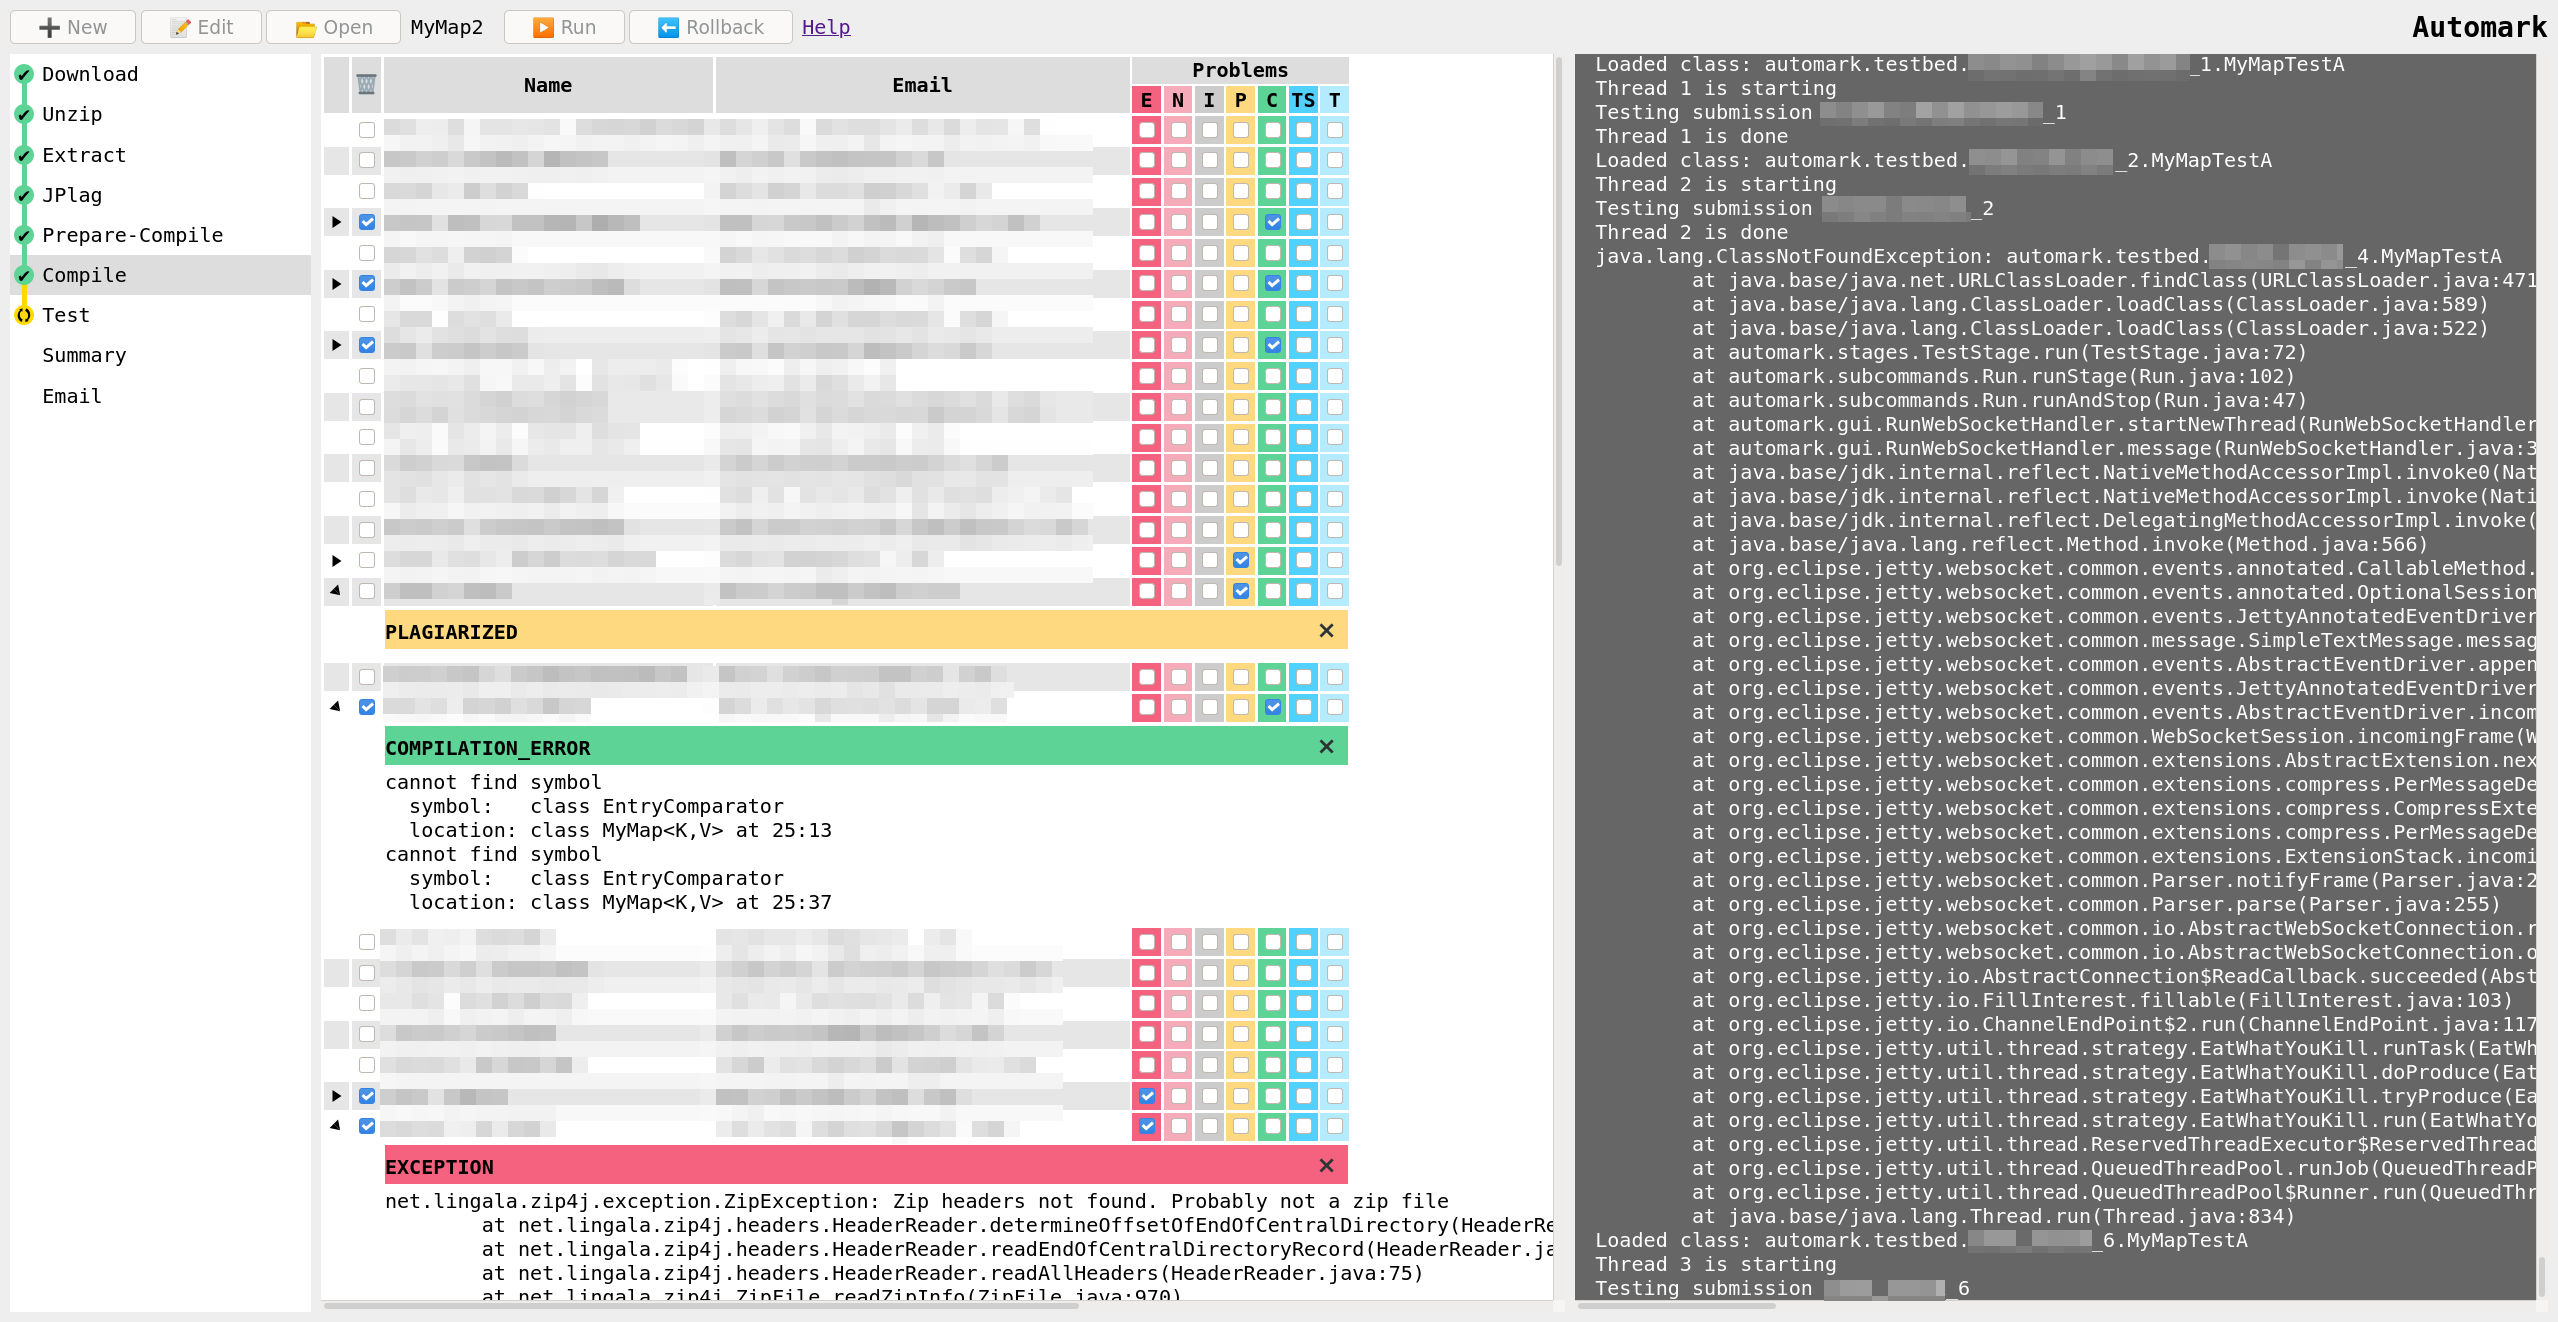
\includegraphics[width=310pt,trim=0pt 0pt 1110pt 0pt,clip]{automark_dashboard_w_details_expanded.png}
			};
			\node at (77,-166) [text width=305,align=center]
				{\emph{Screenshot of Automark's GUI (cropped). The panel on the left-hand side displays an overview over all tasks in the process (\emph{stages}). In the middle there's a table showing an overview as well as detailed information about students' submissions and any problems with them. Personally identifiable information has been blurred.}};
			\node at (77,-220)
				{--};
			\node at (77,-240)
				{Public; Library of the \EmSchoolName};
		}
	}{}
	\clearpage
	\tableofcontents
	\newpage
	\pagenumbering{arabic}
	\chapter{Introduction}
	The Easy Mark One project originated from a dissatisfaction with the workflow of reviewing, grading and communicating assignments in programming classes. Workflows to this date are largely based on repetitive manual labor and rigor which not only makes them error-prone; it also results in many teachers outright (and understandably) skipping this work which can create a net negative for the pupils' education.

	The project aims to fix this issue with two independent software packages: \emph{Automark} and \emph{EasyMark}. Both programs are implemented largely in Java and some other languages like JavaScript, CSS and Pebble\parencite{pebblewebsite} for web-based components.

	\section{Automark}
	Automark is a tool to automate the objective tasks of grading programming assignments. That means it can automatically download, verify, compile and test programming assignment submissions and generate summaries and reports about the status of each submission along the way.

	To achieve its goals of simplicity and high automation, Automark integrates with existing learning management systems (LMS), third party verification tools, compilers and other systems. Despite its deep integration, Automark is built to be highly resilient against failure. The program can handle invalid submissions and unexpected input without crashing; instead it associates errors with the submission it has been processing and notifies the operator and -- optionally -- also the submitter about it.

	Automark employs advanced and up-to-date third party tools for testing and detecting software plagiarism between submissions. In addition to that, it automatically builds a historical database of all submissions for a given assignment to detect plagiarism from previous years' submissions.

	Automark replaces a range of existing tools for its tasks and employs a clean and extensible internal structure. It is perfect for tying together unorganized manual grading workflows.

	\section{EasyMark}
	EasyMark is an online web-based platform for connecting students and teachers and communicating grades and assignment information.

	EasyMark provides teachers with the ability to create courses with chapters and assignments for students to view. Then later on, when a student has completed an assignment and submitted it over another channel (such as Moodle) the teacher can perform an assessment of the submission (for example, via Automark) and enter the results in a user-friendly yet powerful GUI on EasyMark. EasyMark then automatically calculates the new grading status of then student and notifies them the next time they log in.

	Additionally, EasyMark allows students to volunteer for an exam on chapters where the teacher has enabled the feature. The teacher is able to view these test requests on a feature-rich dashboard immediately after logging in.

	Unlike Automark, EasyMark does not aim to replace existing tools (which in this case would be learning management systems like Moodle or WebUntis). Rather, it extends them with new features not available in currently employed LMS solutions and fosters cooperation with existing systems by providing functionality to link to and import from third party platforms such as Moodle.

	EasyMark also employs unparalleled security and data protection features. Personally identifiable information (such as names) are encrypted and only accessible via the teacher's access token. Bad actors who gain access to the server are not able to read the protected information from the database file. In addition to that, EasyMark gives teachers and students deep insight over what happens to their accounts. Teachers and students have the ability to view and revoke currently active sessions on their account. Teachers also see an append-only log of all actions conducted with their account to quickly detect intrusion.

	\iffalse
	\chapter{Quick-Start Guide}
	This chapter is for readers who would like to have a quick development setup for review and assessment. It does not go into detail about the various features of the programs described and the end-result is not ready to be used in a production environment. For production-ready builds and deployment please see one of the later chapters. %TODO: reference production-ready build/deploy chapters

	The guide will often mention an "IDE" (integrated development environment). It should be noted that you do not require an IDE to complete this setup, although it is advisable. The guide sometimes includes special setup instruction for IntelliJ IDEA\parencite{intellijwebsite} hence why it is the recommended IDE for this guide.

	\section{Automark}
	This section guides you through the setup of Automark for development and assessment.

	\subsection{Obtaining the Source}
	The Automark source code can be obtained from the project's GitHub repository using the builtin functionality to clone (download) repositories using the version control system (VCS) Git. Additionally you can use the command line ("Git Bash" on Microsoft Windows, any shell on other systems) with the following command:
	\begin{lstlisting}[language=sh]
		git clone https://github.com/T0astBread/automark
	\end{lstlisting}
	The author does not guarantee availability of the source code repository at this location.

	If you have access to the physical copy of this document you can also obtain the source from the included DVD-ROM.

	\subsection{Opening the Project}
	You can open the project as a normal Gradle project. In IntelliJ IDEA this is the "Open or Import" option on the start screen or the "Open..." option in the "File" dropdown on any other screen. After opening the project a notification will pop up with a link titled "Import Gradle project". Click that link.

	\subsection{Running the Program}
	When running Automark you have two choices: You can use it from the command line or you can use it via the included GUI. To set up a new project or explore features it is recommended you use the GUI, since it provides a simple UI for project creation, configuration and usage.

	\pagebreak
	To run the program you can execute the Gradle task "run" with special options depending on how you intend to run the program. On the command line this can be done with
	\begin{lstlisting}[language=sh]
		./gradlew run --args "<automark args go here>"
	\end{lstlisting}
	in the project directory. On Windows replace "gradlew" with "gradlew.bat".

	You can create an IntellJ IDEA run configuration to execute the task with a single keystroke. To do so, click "Add configuration..." or (if you already have run configurations) click the run configuration drop down and click "Edit configurations...". In the new window, click the plus icon in the top left corner and select "Gradle". In the "Gradle project" field enter "automark", leave the "Task" field blank and instead enter \lstinline|run --args "<automark args go here>"| in the "Arguments" field. Details of the various command line arguments can be found in later chapters. %TODO: reference Automark command line arg chapters

	It is recommended you enter \lstinline|-Dfile.encoding=UTF8 -Dsun.jnu.encoding=UTF-8| in the "VM Options" field to ensure HTML content is rendered correctly for web features.

	To quickly try out features, it is recommended you start the GUI. The subcommand for that is simply "gui" (\lstinline|run --args "gui"|). If your platform supports it (which should be the case for Windows) a browser window will pop up titled "Automark". If your platform lacks support for the Java feature used to implement that an URL will be printed to stdout which you can open in your browser.

	\textbf{Important:} For security reasons, Automark will set a cookie in your browser when you start it and deny requests from browsers that do not have this cookie. You can't use Automark from a browser window or tab other than the one it opened in. If you close that window or tab, you would have to restart the Automark GUI to use it again.

	%TODO: continue this if needed or delete
	\fi

	\chapter{Automark}
	Automark is a tool to automate the task of reviewing programming assignments.

	\section{Technology Used}
	Automark is implemented on top of Java and incorporates various libraries to provide some of its functionality. It has been written using the IntelliJ IDEA IDE and the Gradle build system.

	\subsection{Java} \label{subsec:java}
	Java is a class-based, object-oriented programming language that runs on its own virtual machine (VM) called the JVM and can thus run on any operating system that implements a JVM\parencite{oraclethejavalangenvironment}. The technology was chosen because of the familiarity of the author and the cooperation partner with the language and the (in the field of programming) well-known stability of the language.

	\subsection{Gradle} \label{subsec:gradle}
	Gradle is a system to automate compilation, linking and packaging (in combination referred to as "building") for a variety of languages including Java. In addition to simplifying software builds it also caches results and avoids re-compiling up-to-date compilation units (classes in Java). Gradle is also well-integrated into the IDE used.\parencite{gradlewebsite}

	\subsection{IntelliJ IDEA} \label{subsec:intellijidea}
	IntelliJ IDEA is an integrated development environment (IDE) from JetBrains s.r.o.\parencite{intellijwebsite} An integrated developmentcan be viewed as an advanced text editor that offers convenience features for the programmer, such as syntax highlighting, context-aware code completion, debugging and build integration\parencite{stevenjzeilintegrated}\parencite{idewikipedia}. IntelliJ was chosen because of the author's familiarity and satisfaction with it. The Apache-2.0-licensed Community edition was used.

	\subsection{Libraries}
	Automark uses a few libraries to provide some of its functionality.

	\subsubsection{GSON} \label{subsubsec:gson}
	GSON is a Java library by Google for simple serialization and deserialization of Java objects to and from JSON objects and arrays\parencite{gsongithub}. It was chosen since it operates using Java's reflection feature which spares the developer from having to write explicit parsing code.

	\subsubsection{JSoup} \label{subsubsec:jsoup}
	\BlockCite{jsoup is a Java library for working with real-world HTML. It provides a very convenient API for fetching URLs and extracting and manipulating data, using the best of HTML5 DOM methods and CSS selectors.}{jsoupwebsite}

	JSoup is used for automatically obtaining data from Moodle. Since the Moodle version Automark is built for does not make heavy use of client-side scripting (which JSoup does not support), JSoup was the most stable choice.

	Alternatives to JSoup would typically use a fully-fledged browser such as Google Chrome or Firefox and automate website interactions using APIs (application programming interfaces) provided by the browser which then perfoms interactions as if a human user had done it. Aside from reduced speed, the main drawback with this approach is that library versions quickly become outdated due to the underlying browser version becoming outdated. In the case of some libraries, vendors will not provide downloads for old browser versions anymore leading to breakage of new installations.

	\subsubsection{Zip4j} \label{subsubsec:zip4j}
	Zip4j provides ZIP packing and extraction functionality.\parencite{zip4jwebsite} It is used to unpack submission files downloaded from Moodle or provided by the operator.

	\subsubsection{JUnit 5} \label{subsubsec:junit5}
	JUnit 5 is a unit testing framework for JVM languages.\parencite{junit5website} In Automark it is used for running unit tests provided by the operator against students' submissions. JUnit 5 provides a simple interface for automating test execution via the "junit-platform-launcher" package\parencite{junitplatformlauncherdocs}.

	\subsubsection{Simple Java Mail}
	Simple Java Mail wraps Java's email APIs to improve the developer experience (DX) when sending email\parencite{simplejavamailwebsite}. It is used to send result-email to students after their submissions were tested if enabled by the operator.

	\subsubsection{Spark}
	Spark is a web server framework for JVM languages (with special focus on Java and Kotlin)\parencite{sparkwebsite}. It is used to provide the in-Browser GUI locally and with security restrictions. %TODO: refenrence GUI security restrictions chapter

	\subsubsection{Preact} \label{subsubsec:preact}
	Preact is a \emph{Fast 3kB alternative to React with the same modern API}\parencite{preactwebsite}. It is used to simplify the user interface logic in complex web applications which results in cleaner code and less UI bugs. Preact in particular was chosen over its competitors like React because of its ease of integration.

	\pagebreak
	\subsection{JPlag} \label{subsec:jplag}
	\BlockCite{JPlag is a system that finds similarities among multiple sets of source code files. This way it can detect software plagiarism. JPlag does not merely compare bytes of text, but is aware of programming language syntax and program structure and hence is robust against many kinds of attempts to disguise similarities between plagiarized files.}{jplagwebsite}

	JPlag is incorporated as a pre-built JAR file that gets written to disk and started via Java's ProcessBuilder API when needed. The JAR file is also tracked as a binary file in the VCS since JPlag could -- at the time of writing -- not be built from source independently.

	JPlag is only used in the \lstinline|JPLAG| stage. See \ref{subsubsec:jplag}~JPLAG.

	\section{Functionality}
	Automark is used to automate the process of grading programming assignments in the programming language Java as far as possible and with superior stability. To facilitate this, Automark employs a design that seperates the process of reviewing assignments (called "pipeline") into multiple tasks (called "stages"). Each stage is dependent on the result of the respective previous stage.

	Stages are run without manual intervention unless required. If a submission fails to fulfill the requirements of a stage, it will be tagged with a so-called "problem" and possibly excluded (if the specific problem renders the submission unfit for further processing). If a stage completes, Automark will automatically continue with the next stage, unless a problem has been detected in at least one submission during the stage.

	After a stage completes with new problems in submissions the operator should review the problems and do one of the following to each:
	\begin{itemize}
		\item \textbf{Leave the problem be} if it is justified.
		\item Use the \textbf{Rollback} feature to revert the completed stage. The operator can then adjust the output of the previous stage to correct any mistakes that cause the stage to output unwanted problems.
		\item Use the \textbf{mark-resolved} subcommand to remove one or more problems from the database without actually changing the submission data.
	\end{itemize}

	\subsection{Problems}
	Automark categorizes failures of submissions to meet requirements as problems of different types.

	\begin{description}[align=left]
		\item[EXCEPTION] Denotes that a Java exception was thrown while processing the submission. This most frequently occurs due to invalid or malformed input in submissions.
		\item[NOT\_SUBMITTED] Denotes that while it was captured that the student has been added to the assignment the student did not submit a solution.
		\item[INVALID\_SUBMISSION\_FILE] Used to report a variety of problems with the submission file(s) that were not captured as a Java exception during processing.
		\item[PLAGIARIZED] Denotes that a submission contains similarities with another submission of the same assignment or a submission of the assignment from a previous year. This problem type is not assigned automatically. See \ref{subsubsec:jplag}~JPLAG.
		\item[COMPILATION\_ERROR] Denotes that the Java compiler reported one or more errors while compiling the source files in the submission. If the compiler reports errors while compiling the operator-provided test suites with the sources it is not reported as a \lstinline|COMPILATION_ERROR| but rather as a \lstinline|TEST_SUITE_FAILURE|.
		\item[TEST\_SUITE\_FAILURE] Denotes that, during the \lstinline|TEST| stage, a whole test suite either was not completed (for example due to a timeout) or was not started in the first place (for example due to a compilation error).
		\item[TEST\_FAILURE] Denotes a failure of a JUnit test during the \lstinline|TEST| stage on the given submission.
	\end{description}

	In addition to the type a problem also includes a summary which contains either a short description or detailed diagnostic information such as a stacktrace. In case of the latter it will be shortened in reports sent out to students. Problems also record in which stage they occured.

	\subsection{Stages}
	Automark seperates the processing pipeline into nine stages. This section enumerates the stages and explains their implementation (in order of execution).

	\subsubsection{DOWNLOAD}
	The \lstinline|DOWNLOAD| stage is not an actual stage but rather a hyperonym to refer to either the \lstinline|BypassDownloadStage| or the \lstinline|MoodleScraperStage|. The whole program refers to them using the term \lstinline|DOWNLOAD| with the only exception being the configuration wizard.

	\subsubsection{MoodleScraperStage}
	This stage takes Moodle credentials (of the operator) as its parameters among others. It logs into Moodle, obtains the names and email addresses of students added to the assignment and checks if a submission is present. If it is, it is downloaded. If it is not, a \lstinline|NOT_SUBMITTED| problem is added to the submission entry for the student and it is excluded from further processing.

	The web scraping features in this stage are implemented using the JSoup library (see \ref{subsubsec:jsoup}~JSoup). JSoup is augmented to store cookies from server responses to implement sessions.

	\subsubsection{BypassDownloadStage}
	This stage is an alternative to the \lstinline|MoodleScraperStage| and is mainly designed as an emergency solution if the \lstinline|MoodleScraperStage| breaks, for example due to an incompatible change on the Moodle website.

	The \lstinline|BypassDownloadStage| obtains submissions and metadata from a ZIP file which the operator can download from Moodle manually using the "Download all submissions" ("Alle Abgaben herunterladen" in German) option in the grading editor.

	The stage optionally reads in a file called "emails.csv" which is a comma-separated values (using semicolons as separators) file in the format \lstinline|Moodle name;email address| which it uses to map email addresses to submissions for potential later use in the \lstinline|EMAIL| stage. The lines in the file do not have to map exactly to the names in the "all submissions" ZIP file.

	Normally the \lstinline|BypassDownloadStage| does not mark missing submissions as \linebreak\lstinline|NOT_SUBMITTED| since the "all submissions" ZIP file from Moodle does not contain any information from which the stage could infer that a student who has not submitted a solution exists. However, if an "emails.csv" file is present and the file contains one or more lines with names that do now match any submission, then the \lstinline|BypassDownloadStage| will create submission entries for those students, mark them as \lstinline|NOT_SUBMITTED| and exclude them from further processing.

	\subsubsection{UNZIP}
	This stage simply unpacks submissions, which are expected to be ZIP files at this point. If submissions are not ZIP files or otherwise incompatible with the Automark unzipping mechanism they are marked with an \lstinline|EXCEPTION| problem and excluded from further processing. If the file does not exist at all it is also marked with an \linebreak\lstinline|INVALID_SUBMISSION_FILE| problem.

	ZIP files are processed using zip4j. See \ref{subsubsec:zip4j}~Zip4j.

	\subsubsection{EXTRACT}
	Reads the \lstinline|sourceFiles| parameter from the config file which holds a comma-seperated list of Java file names and filters files in submissions recursively for these file names. If a submission does not contain any of the wanted files it is marked with the \linebreak\lstinline|INVALID_SUBMISSION_FILE| problem and excluded from further processing.

	\subsubsection{JPLAG} \label{subsubsec:jplag}
	This stage's main objective is running the JPlag program (see \ref{subsec:jplag}~JPlag) to detect structural similarities between submission of the current assignment and with submissions of the same assignment from previous years.

	To achieve this, it maintains a historical database (called the "JPlag repository") of all submissions for a given assignment over multiple years. Assignments are identified by their name (the \lstinline|assignmentName| parameter in the config file) since Moodle's assignment ID will probably change between years (since new courses are created with new assignments from Moodle's point of view). At the end of the \lstinline|JPLAG| stage all submissions are copied to the JPlag repository. The location of the JPlag repository is determined by the \lstinline|jplagRepository| parameter in the config file. It is recommended to use an absolute file path for this parameter but relative file paths are also possible.

	The stage will not mark plagiarized submissions with the \lstinline|PLAGIARIZED| problem automatically. JPlag's detection is not accurate enough to facilitate this in all cases and parsing JPlag's generated report would be cumbersome. Instead, execution is explicitly halted after the \lstinline|JPLAG| and the generated JPlag report is opened in a browser (if the system supports it) for the operator to review. The \lstinline|JPLAG| stage and the \lstinline|SUMMARY| stage are the only stages that always halt execution.

	If the \lstinline|JPLAG| stage is rolled back the JPlag repository will not be rolled back. It is the responsibility of the operator to keep the repository clean. If there is a clash between a submission in the repository and a submission in the current project (because the submission has already been copied to the repository), the submission from the repository will override the submission from the current project and nothing will be copied back to the repository. Submissions in the repository are contained in a single directory each in the folder of the current assignment. The submission folder follows the naming scheme "yyyy\_student\_slug" (see \ref{subsec:slugs}~Slugs). Deleting the submission folder is enough to remove the submission from the repository.

	\subsubsection{PREPARE\_COMPILE}
	In Automark, submissions are compiled in and loaded into the same JVM that Automark itself is running in. To avoid name clashes the \lstinline|PREPARE_COMPILE| stage assigns a unique package name to each submission and moves the submission's classes and a copy of all test suites to that package. Test suites are provided by the operator as Java files in a folder called "tests" at the project root and should contain a package header, although the package name doesn't matter. Classes are moved to the namespaced package by searching for and replacing the existing package header in the submission's Java files, then writing the new file contents to a file in the correct folder hierarchy for the package (since that's important for the Java compiler and class loader).

	This stage could have been collapsed with the \lstinline|COMPILE| stage but it has been kept separate since it might be a good intervention point if something goes wrong with, for example, the package header patching and the operator needs to manually correct submission files (although in testing that never happened).

	\subsubsection{COMPILE}
	This stage invokes the Java compiler to compile the submission's source files. It first only runs on the source files provided by the student. Compilation errors after this phase are reported as \lstinline|COMPILATION_ERROR| problems and the submission is excluded from further processing. Afterwards, the compiler is run again on both the student's source files as well as the operator-provided test suites. Compilation errors in this phase are only logged to stdout for diagnostics but not marked as problems. However, if a test suite fails to compile, it will later be reported as a \lstinline|TEST_SUITE_FAILURE| in the \lstinline|TEST| stage due to the class loader being unable to load a class file that does not exist.

	\pagebreak
	A useful benefit of the Java compiler is that even when the compilation includes errors, it still successfully compiles classes that aren't affected by those errors. This allows Automark to, for example, compile and run test suites even when other test suites failed to compile. It is therefore recommended that operators split tests into relatively small test suites.

	\subsubsection{TEST}
	The \lstinline|TEST| stage's main objective is to load all classes in a submission and start JUnit via the junit-platform-launcher API (see \ref{subsubsec:junit5}~JUnit~5). JUnit then finds test suite classes automatically and executes the contained tests. Automark captures test results using the TestExecutionListener interface provided by JUnit to hook into the test execution cycle.

	The stage also reads in all test suite sources (from the "tests" folder) prior to running JUnit and searches for test annotations and method names. From this information it builds a list of all available tests. This has the benefit of improving the reliability of reported results since the source of truth for the list of all existing tests is now independent of what JUnit finds. Additionally Automark uses this opportunity to provide operators with the ability to add descriptions to tests by simply adding a line-commend (\lstinline|//| in Java) in the line after the test annotation. With such a description a test declaration might look like this:

	\begin{lstlisting}[language=java]
		@Test
		// Tests if `put(...)` works with a new key
		public void b1_testPut_newKey_emptyMap() {
			// bla bla bla...
		}
	\end{lstlisting}

	Test descriptions are optional. Regular JUnit 5 test declarations work as well. Test descriptions are included as summaries in \lstinline|TEST_FAILURE| problems and are thus reported to students if report email is sent.

	\subsubsection{SUMMARY}
	The summary stage generates the reports sent out to students if the \lstinline|EMAIL| stage is used. It is broken out into a separate stage to give operators a chance to review and alter the mail that's about to be sent. For this reason execution is also explicitly halted after the \lstinline|SUMMARY| stage (the \lstinline|SUMMARY| stage can in fact not even generate new problems in submissions). The \lstinline|JPLAG| stage and the \lstinline|SUMMARY| stage are the only stages that always halt execution.

	\subsubsection{EMAIL} \label{subsubsec:email}
	The \lstinline|EMAIL| stage is optional and can be turned on or off via the boolean parameter \lstinline|emailStageEnabled| in the config file. If not enabled, it does nothing and immediately finishes. If enabled, it first tries to connect to the SMTP server specified in the config using the following parameters:
	\begin{description}[align=left]
		\item[smtpHost] The hostname of the SMTP server
		\item[smtpPort] The port of the SMTP server
		\item[smtpProtocol] Must be one of:
			\begin{itemize}
				\item \textbf{SMTP:} Plain-text SMTP with an optional STARTTLS upgrade \\if supported by the server
				\item \textbf{SMTPS:} SMTP over TLS; \textbf{This is the recommended option.}
				\item \textbf{SMTP\_TLS:} Initially plain-text SMTP with a mandatory \\STARTTLS upgrade
			\end{itemize}
		This parameter is based on Simple Java Mail's TransportStrategy enum type. See \href{http://www.simplejavamail.org/configuration.html#section-transport-strategies}{Simple Java Mail - Configuration § Transport strategies} for more information.
		\item[smtpUsername] The username to use when connecting to the SMTP server; Can be blank, in which case Automark will prompt the operator for the value when executing the stage.
		\item[smtpPassword] The password to use when connecting to the SMTP server; Can be blank, in which case Automark will prompt the operator for the value when executing the stage.
		\item[smtpFromAddress] The email address to display in the "From" header of outgoing email; This is always required even if only one email address is available to the SMTP account.
		\item[smtpFromName] The name to display in the "From" header of outgoing email; This is always required even if only one email address is available to the SMTP account.
	\end{description}

	Then the \lstinline|EMAIL| stage sends each report generated by the \lstinline|SUMMARY| stage as an email to the student. If a student is not associated with an email address, the submission will be marked with an \lstinline|EXCEPTION| problem.

	Rolling this stage back has no real effect. If this stage fails midway through sending reports out to students, it is recommended the operator deletes all reports already sent from the summary folder before running the \lstinline|EMAIL| stage again to avoid double-mail for some students. Which reports have already been sent can be seen in stdout.

	\subsection{Slugs} \label{subsec:slugs}
	To avoid name collisions, submissions are internally referred to using so-called "slugs", i.e. human-readable unique identifiers. Submission slugs in Automark consist of the student name in snake case (fully lowercase, underscores replace spaces) concatenated with another underscore and an arbitrary unique but humanly comprehensible number. Automark assigns these numbers consecutively when it initially creates submission entries.

	\subsection{Config File}
	Each assignment directory must contain a file called "config.properties", referred to as the config file. In the GUI such a file can be created via the "New Assignment" screen. The CLI does not have a builtin way of bootstrapping an assignment, so operators using the CLI would either have to write the config file themselves, copy a previous config file and adjust it or use the GUI to create the config file.

	The config file is in the Java properties file format which is -- in simplified terms -- a list of key-value pairs separated by an equals sign (\lstinline|=|).

	An example config file might look like this:
	\begin{lstlisting}
		assignmentName=MyMap
		assignmentID=27815
		jplagLanguage=java17
		jplagRepository=/path/to/repo
		downloadStage=moodle
		moodleBaseURL=https\://my-moodle-site.org/myschoolname
		moodleUsername=myuser123
		moodleTeachers=teacher1@school.org teacher2@school.org
		sourceFiles=MyMap.java, Entry.java, Node.java
		emailStageEnabled=true
		smtpHost=127.0.0.1
		smtpPort=3025
		smtpUsername=foo
		smtpProtocol=SMTPS
		smtpFromAddress=automark@local
		smtpFromName=Automark
	\end{lstlisting}

	\subsubsection{Config File Options}

	\begin{description}
		\item[downloadStage] The download stage to use; Possible values: \lstinline|moodle| or \lstinline|bypass|
		\item[assignmentID] Numeric assignment ID given to the assignment by Moodle
		\item[assignmentName] Any name by which the operator will recognize the assignment;\linebreak{}Not tied to Moodle
		\item[jplagLanguage] The language setting to use for JPlag (see \lstinline|jplag --help|)
		\item[jplagRepository] The directory to use as the JPlag repository; Relative paths are possible but absolute paths are recommended.
		\item[moodleBaseURL] The URL of your Moodle's login page minus the trailing \lstinline|/login/index.php|
		\item[moodlePassword] The operator's Moodle password; \textbf{Optional:} The operator will be asked for it if it hasn't been provided upfront.
		\item[moodleTeachers] Email addresses of teachers in the Moodle course of the assignment; No email will be sent to these addresses. They are merely required to filter the Moodle accounts of teachers from the pipeline.
		\item[moodleUsername] The operator's Moodle username; \textbf{Optional:} The operator will be asked for it if it hasn't been provided upfront.
		\pagebreak
		\item[sourceFiles] Comma-seperated list of Java files to regard as part of the assignment and use for testing
		\item[emailStageEnabled] Boolean value; whether to enable the \lstinline|EMAIL| stage
		\item[smtpHost] See \ref{subsubsec:email}~EMAIL
		\item[smtpPort] See \ref{subsubsec:email}~EMAIL
		\item[smtpUsername] See \ref{subsubsec:email}~EMAIL
		\item[smtpPassword] See \ref{subsubsec:email}~EMAIL
		\item[smtpProtocol] See \ref{subsubsec:email}~EMAIL
		\item[smtpFromName] See \ref{subsubsec:email}~EMAIL
		\item[smtpFromAddress] See \ref{subsubsec:email}~EMAIL

	\end{description}

	\section{User Interface}
	Automark can be used both via the command line and over a GUI. The command line interface (CLI) was implemented first and is well-suited for integrating Automark into other automation workflows or for users who prefer the command line. The GUI was added later as a means to flatten the learning curve for new adopters, however some users might find they are faster with the GUI.

	Functionally, the GUI and the command line are equal except that the GUI includes a powerful configuration editor for intuitive creation and editing of assignment configurations. There is no analogy for that in the CLI. CLI users can either write the configuration file themselves (or partially re-use previous configuration files) or temporarily use the GUI to generate it.

	\subsection{Command-Line Interface}
	Automark's command-line interface is designed to be non-interactive as much as possible. "Non-interactive" means the running process will not ask for input via stdin but rather read all of its parameters from the command-line and if it needs additional parameters the user has to run the program with those parameters. This style of usage is standard practice for command-line programs as it enables easier automation via (shell) scripting.

	The CLI is partitioned into several subcommands with specific options and some common options.

	\subsubsection{Subcommands}
	\begin{description}
		\item[run] Starts execution from the last completed stage

		This is also the default subcommand when no subcommand is specified.

		\textbf{Syntax:}\tabto{75pt}\lstinline|automark [run]|

		\pagebreak
		\item[status] Displays details about the current state of submissions

		\textbf{Syntax:}\tabto{75pt}\lstinline|automark status|

		\item[rollback] Deletes the results of every stage after \emph{and including} a specified target stage and marks these stages as not completed

		A rollback does not revert global state like the JPlag repository or sent email.

		\textbf{Syntax:}\tabto{75pt}\lstinline|automark rollback <stage>|\\
		\textbf{Arguments:}\tabto{75pt}\lstinline|<stage>| is the name of the target stage (for example \lstinline|COMPILE|)
		\item[mark-resolved] Marks one or more problems in one or more submissions as resolved without actually changing anything about the submission

		Works after every stage but only affects the results of the most recently completed stage so if the operator rolls back, this will be reverted.

		\textbf{Syntax:}\tabto{75pt}\lstinline|automark mark-resolved <slug> [--problem <ident>]|
		\tabto{75pt}\lstinline|  [--requalify]|\\
		\textbf{Arguments:}\tabto{75pt}\lstinline|<slug>| is the slug of the submission to operate on or \lstinline|_| (underscore) to operate on all submissions.

		\lstinline|--problem <ident>| must be present if the operator wants to mark one or more problems as resolved. \lstinline|<ident>| is either the name of the problem (for example \lstinline|EXCEPTION| to match \lstinline|EXCEPTION| problems) or the numerical position of a single problem in the output of automark status. If a problem name is specified, all matching problems are marked as resolved.

		\lstinline|--requalify| must be present if the operator wants to re-include a submission that has been excluded from further processing due to a critical problem.

		mark-resolved without either \lstinline|--problem| or \lstinline|--requalify| is a no-op.

		\item[mark-plagiarized] Tags one or more submissions with the \lstinline|PLAGIARIZED| problem

		Works after every stage but only affects the results of the most recently completed stage so if the operator rolls back, this will be reverted.

		Can be reverted using mark-resolved.

		\textbf{Syntax:}\tabto{75pt}\lstinline|automark mark-plagiarized <slugs>|\\
		\textbf{Arguments:}\tabto{75pt}\lstinline|<slugs>| is one or more space-seperated submission slugs to mark as plagiarized (see \ref{subsec:slugs}~Slugs). Note that this parameter might have to be in quotes (\lstinline|"|) to specify more than one slug, depending on the shell used.

		\item[gui] Starts the GUI

		\textbf{Syntax:}\tabto{75pt}\lstinline|automark gui|

		\item[manual] Shows a manual similar to this chapter in the browser

		\textbf{Syntax:}\tabto{75pt}\lstinline[mathescape]!automark <manual|--help|-h>!
	\end{description}

	\pagebreak
	\subsubsection{Common Options}
	To this date there is only one option that is usable regardless of the subcommand (excluding debug options) and that is \lstinline|--workingDir| or \lstinline|-d| for short. This option sets the working directory for Automark. Usually the operator would run Automark in the directory of an assignment (where the assignment config file is). \lstinline|--workingDir| allows operators to run Automark from a different directory than the assignment directory.

	\subsection{GUI}
	The GUI was developed after the CLI so it simply acts as a wrapper to invoke the same subcommands that are also available in the CLI, for the most part. However, it doesn't look like a typical "CLI wrapper"-style GUI since it cleverly works around that using an easy-to-grasp information-dense design.

	\begin{figure}[h]
		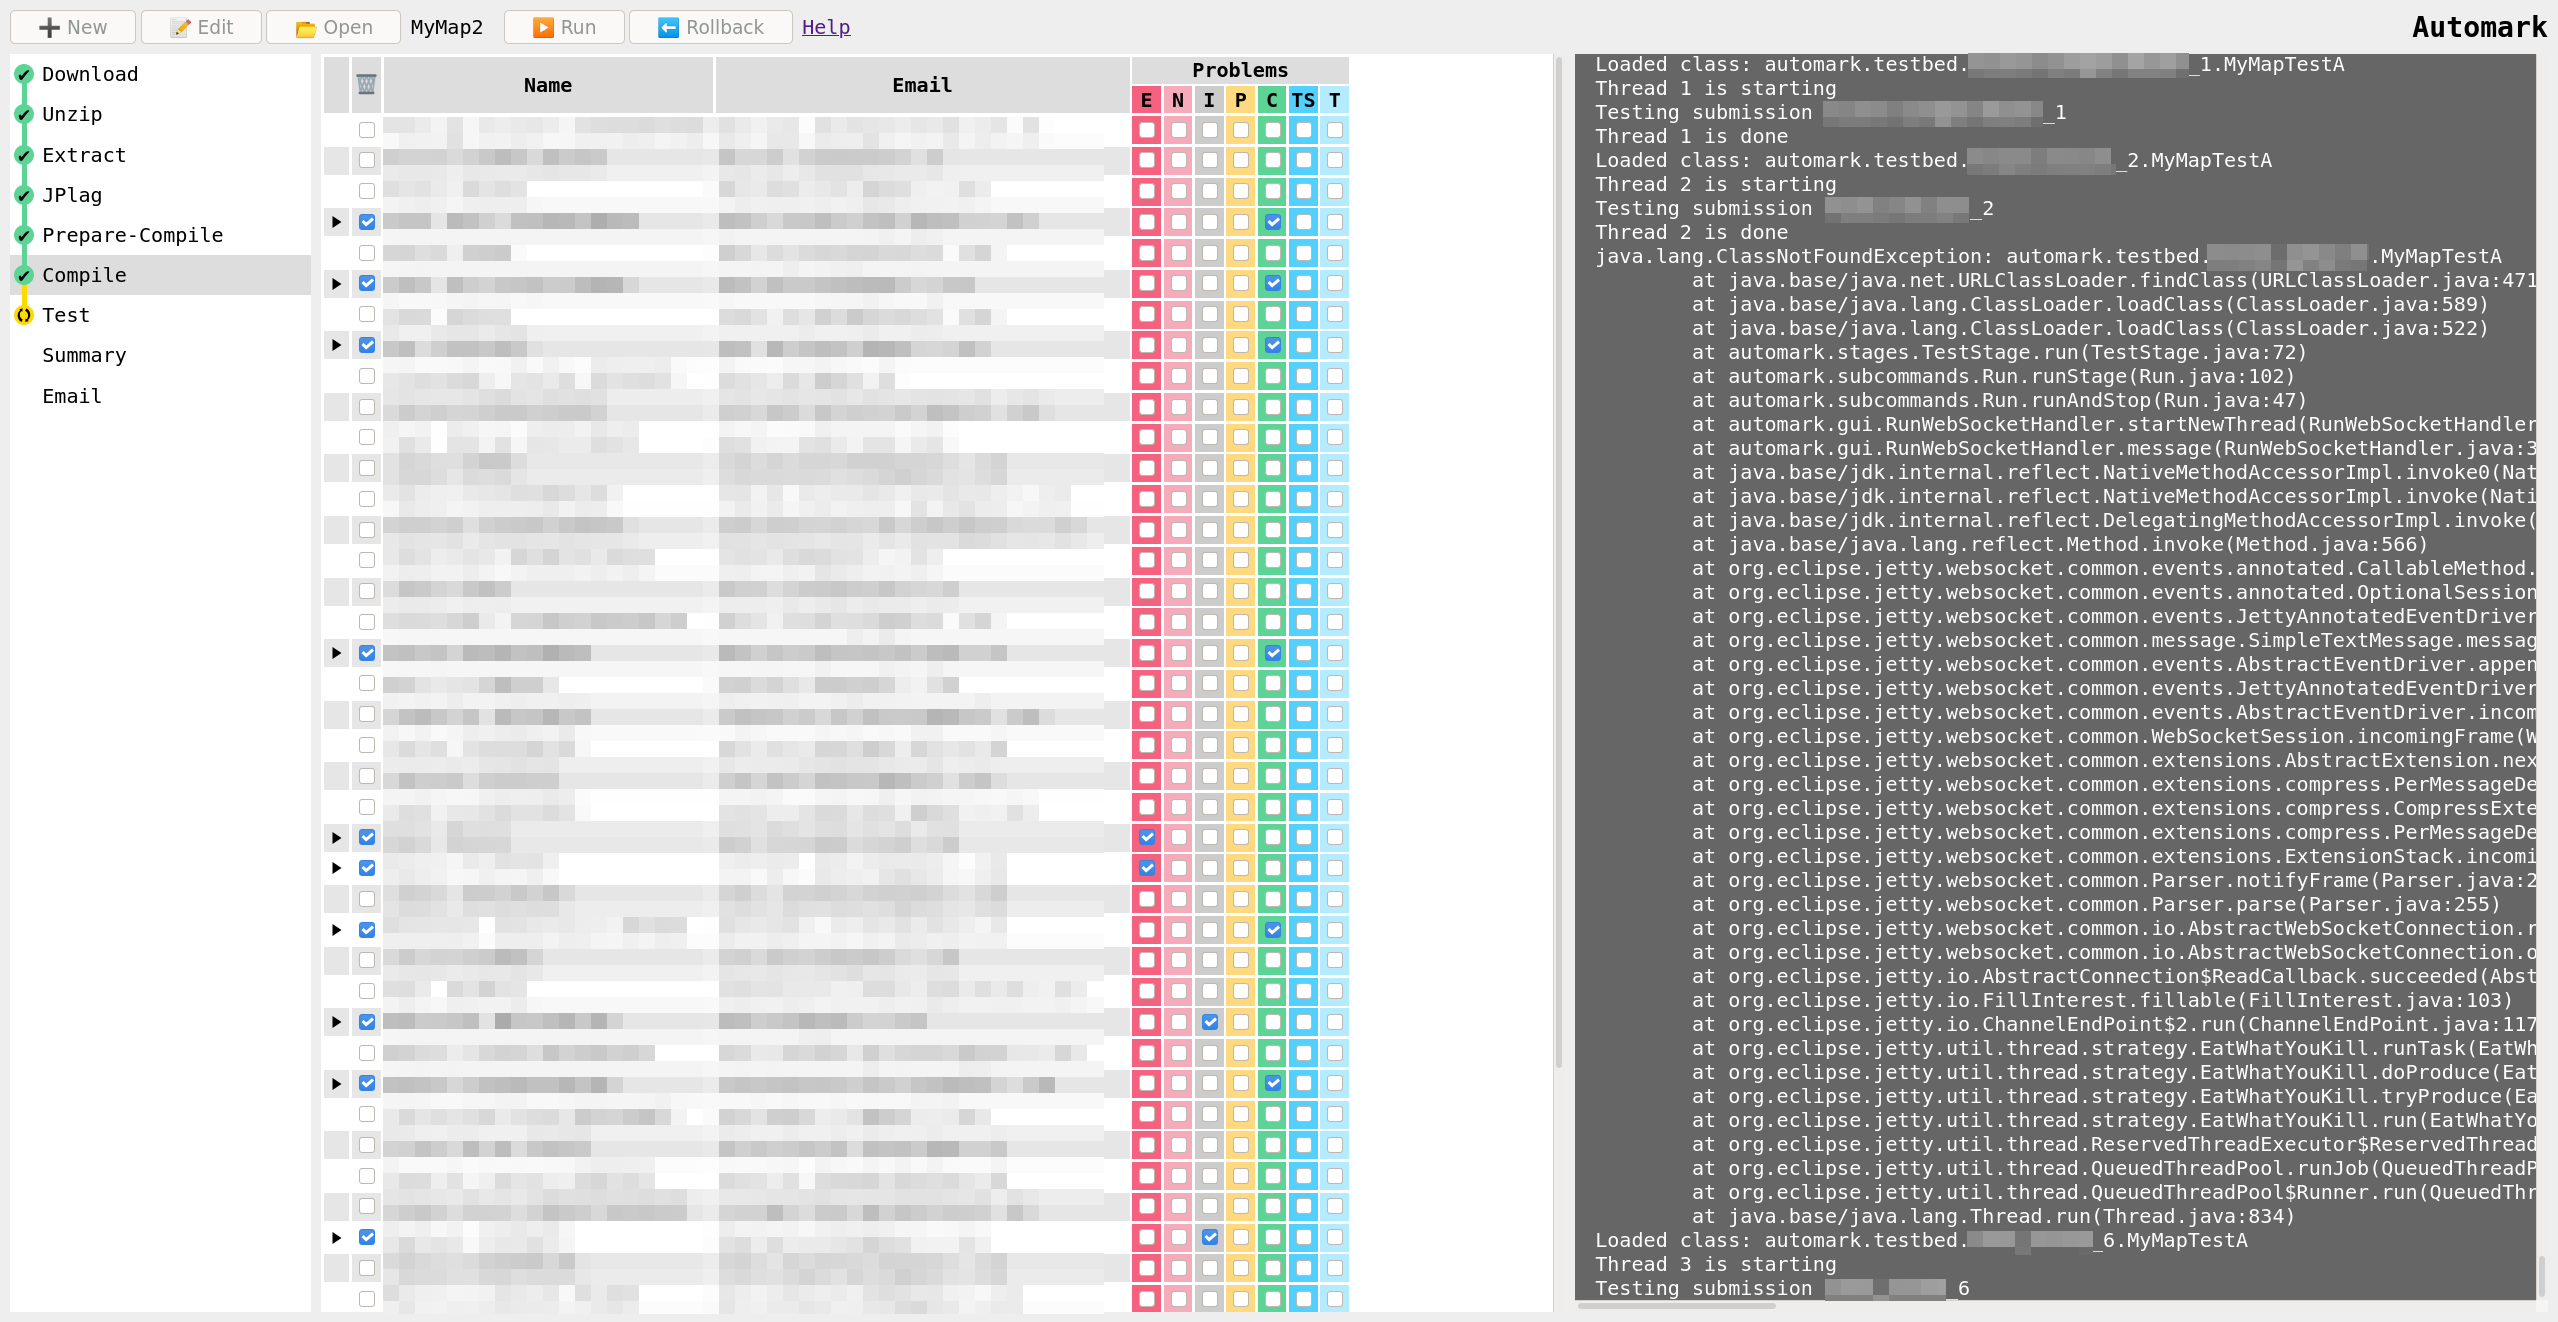
\includegraphics[width=\textwidth]{automark_dashboard.png}
		\vskip0pt
		\caption{Screenshot of the Automark dashboard running the \lstinline|TEST| stage; Personally identifiable information has been blurred.} \label{fig:automarkdashboard}
	\end{figure}

	The GUI consists of several main components which this chapter aims to explain further.

	\pagebreak
	\subsubsection{Start Screen}
	The start screen is only visible when Automark is not started in an assignment directory. It provides access to the configuration editor as the "New Assignment" screen and the "Open" dialog.

	\begin{figure}[H]
		\centering
		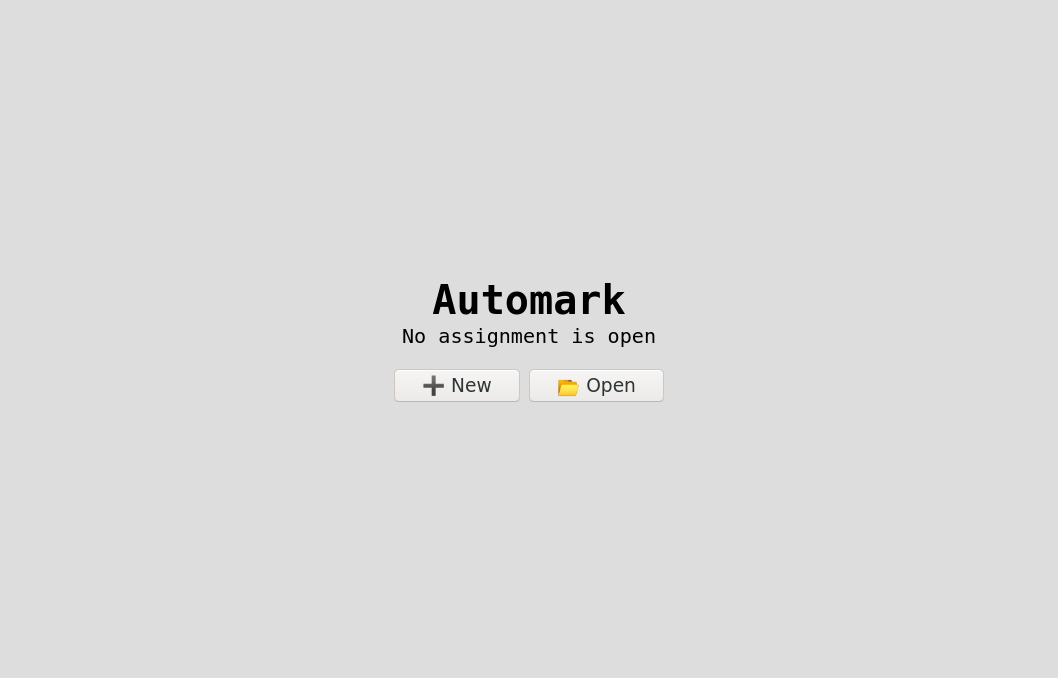
\includegraphics[width=10cm]{automark_start_screen.png}
		\caption{Automark start screen}
	\end{figure}

	\subsubsection{Dashboard}
	The dashboard is the main screen of Automark. It displays information about submissions and lets the operator interact with them. See \autoref{fig:automarkdashboard}.

	\subsubsection{Toolbar}
	The toolbar holds some of the most frequently used functionality in Automark.

	\begin{figure}[h]
		
\includegraphics[width=\textwidth]{automark_toolbar.png}
		\vskip0pt
		\caption{Automark toolbar on an assignment called "MyMap"}
	\end{figure}

	From left to right: \textbf{New} and \textbf{Edit} both open the configuration editor, in the case of the former as the "New Assignment" screen, in the case of the latter as the "Edit Assignment" screen. \textbf{Open} opens the "Open" dialog. \textbf{Run} and \textbf{Rollback} correspond to their CLI counterparts.

	\pagebreak
	\subsubsection{Configuration Editor}
	The configuration editor provides a way for the operator to edit and create config files that is more user-friendly than writing the files by hand.

	It is available in two variants for the "New Assignment" and the "Edit Assignment" screens.

	\begin{figure}[h]
		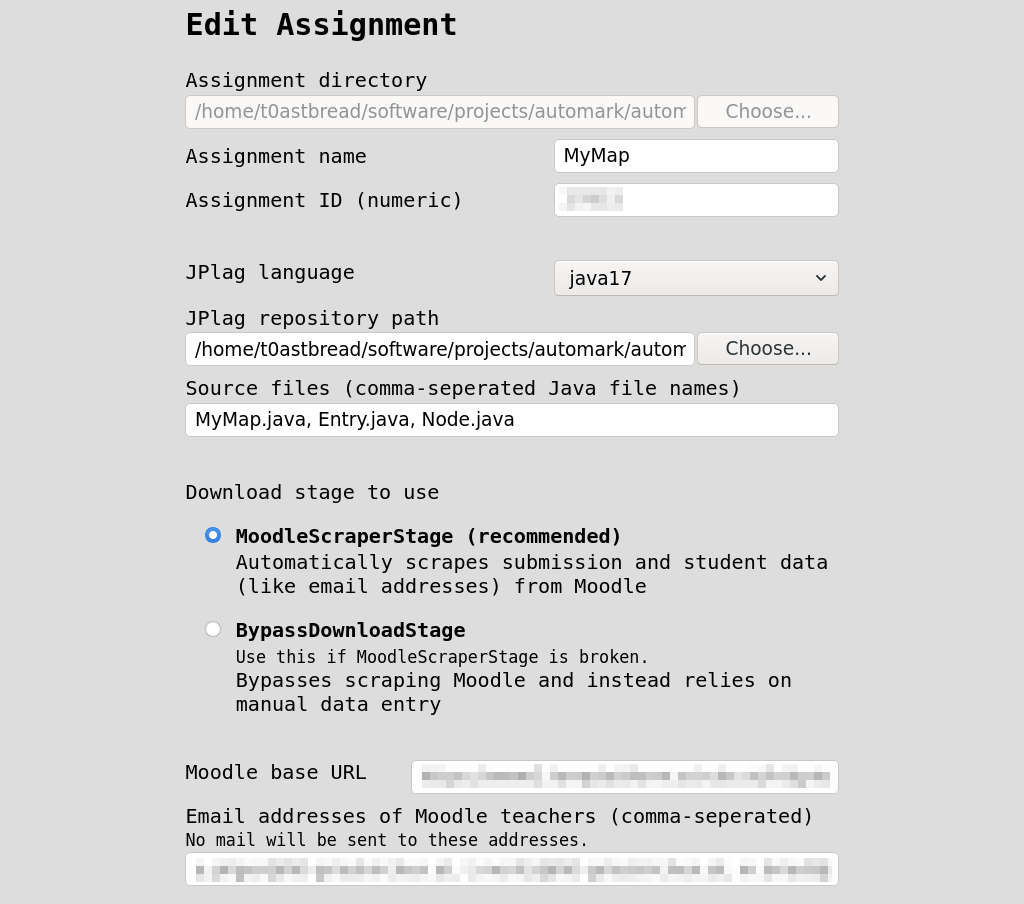
\includegraphics[width=\textwidth]{automark_configuration_editor.png}
		\vskip0pt
		\caption{Cropped screenshot of the configuration editor seen as the "Edit Assignment" screen}
	\end{figure}

	\subsubsection{Open Dialog}
	The open dialog is a simple file picker for directories to switch the active assignment.

	\pagebreak
	\subsubsection{Stage List}
	The stage list is the leftmost component of the dashboard. It displays the current status of completed and running stages and allows the operator to switch the stage results displayed in the submissions table.

	\begin{figure}[h]
		\centering
		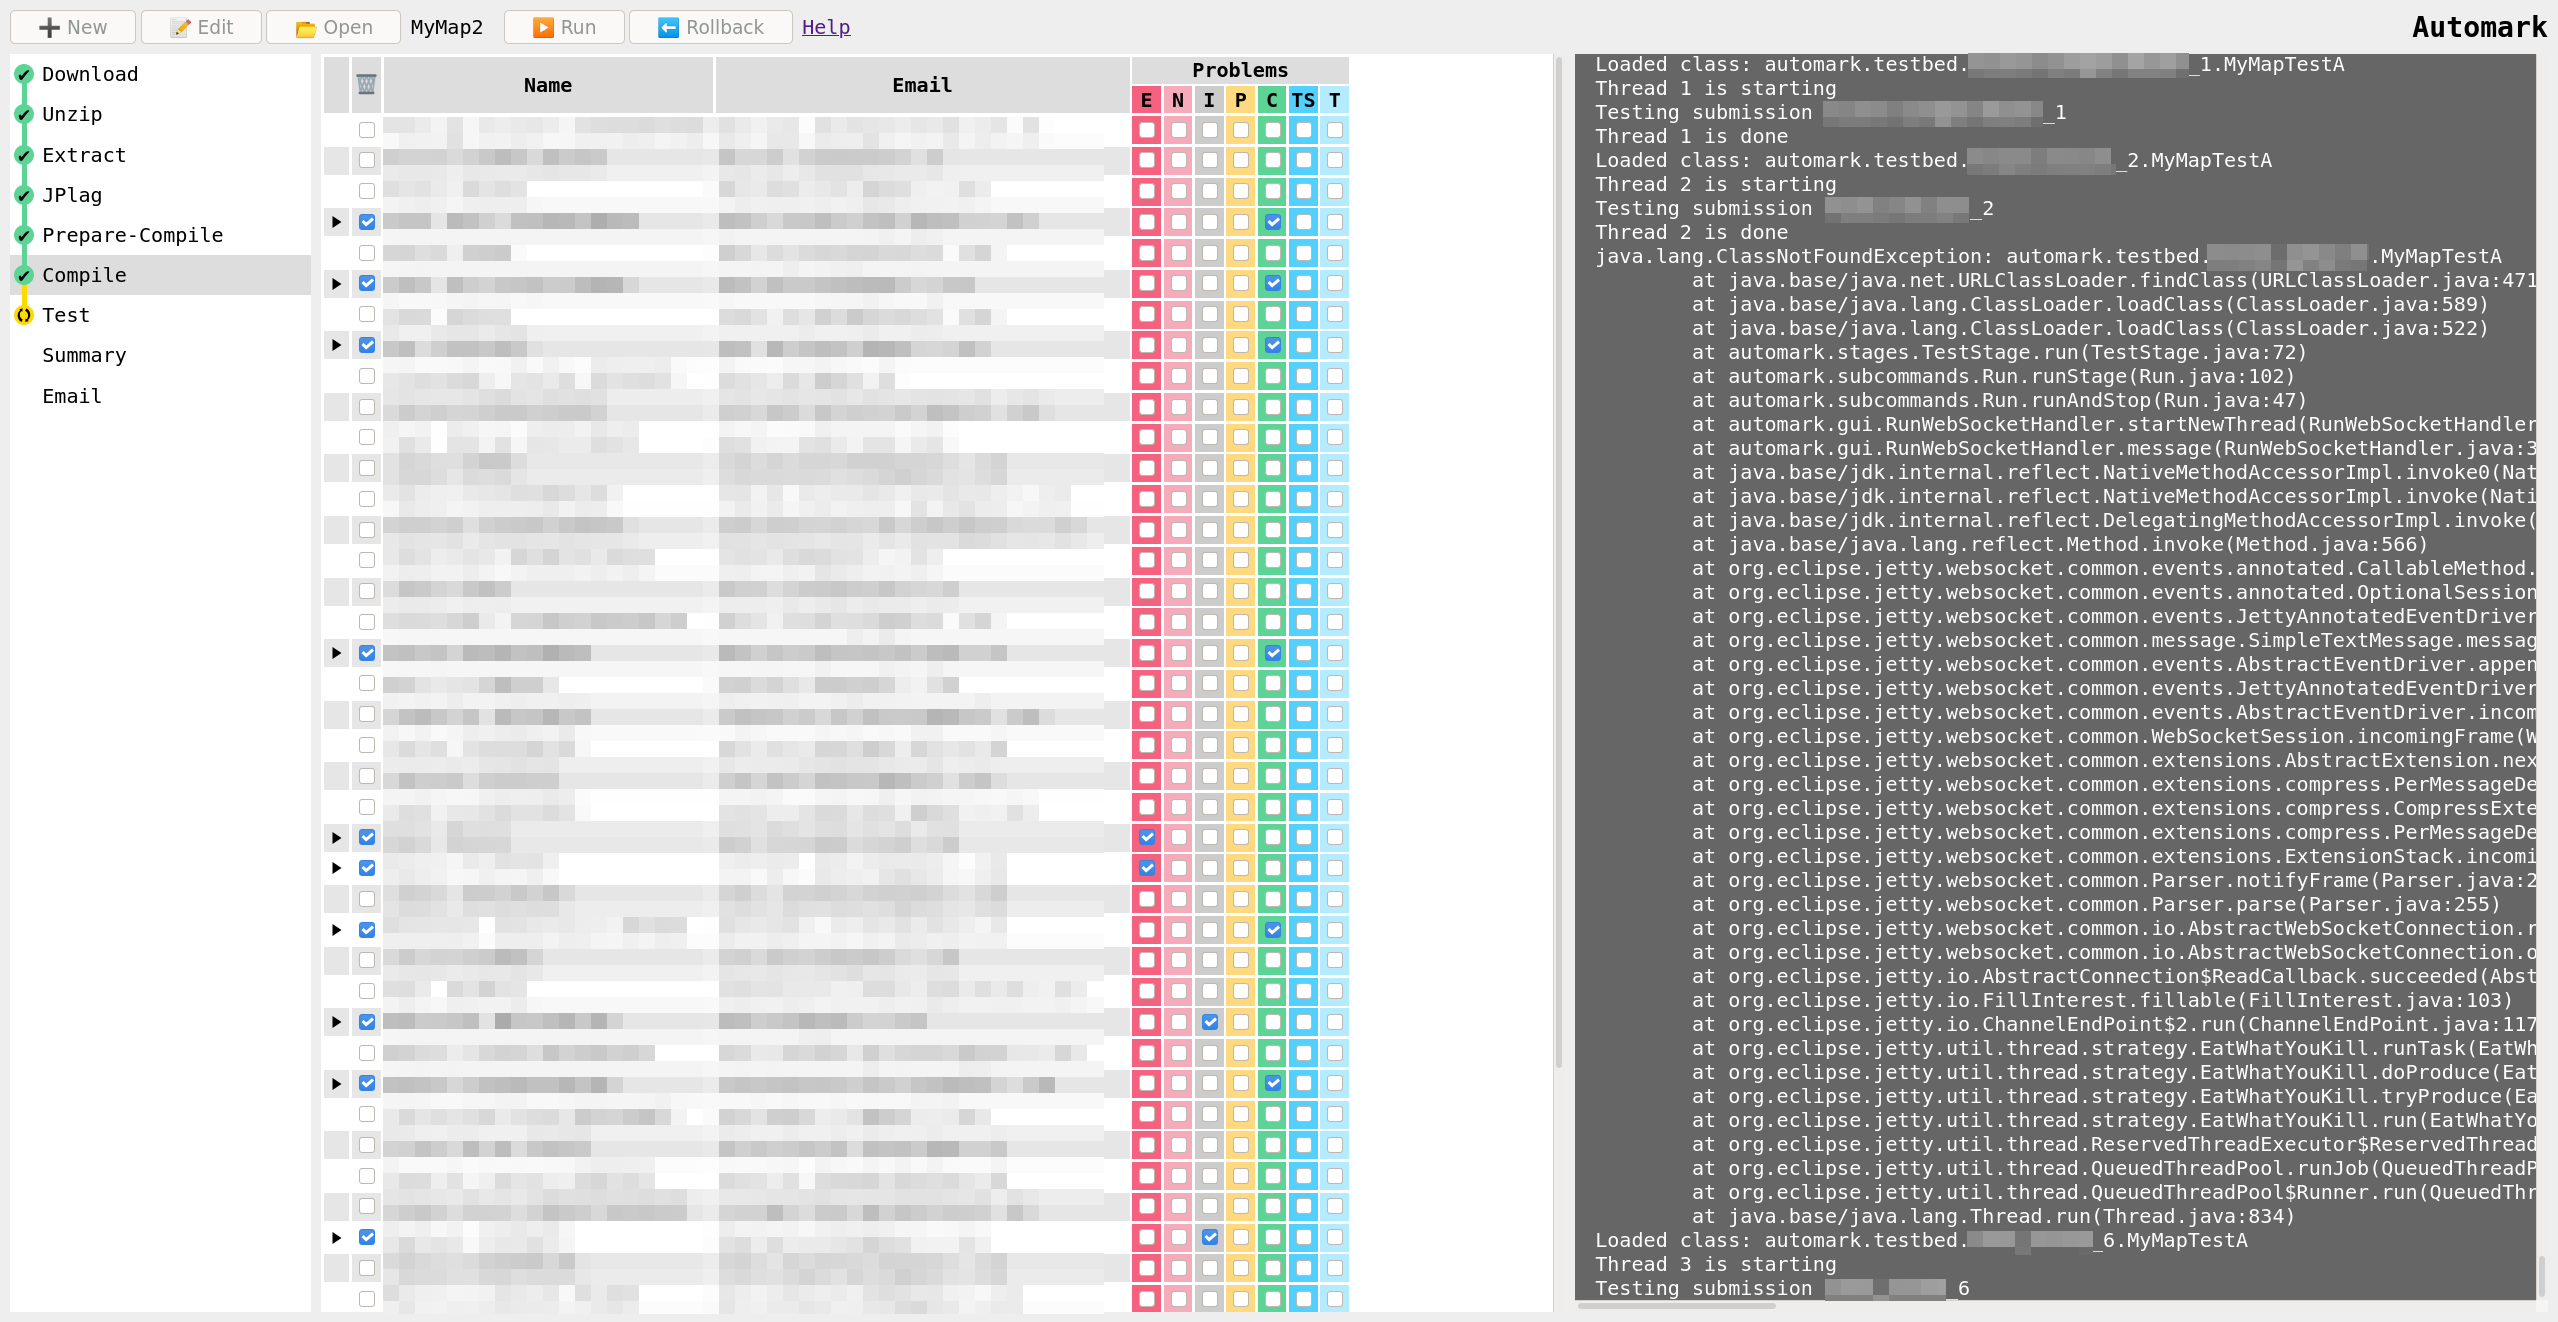
\includegraphics[width=5cm,trim=0 30cm 78.9cm 1.5cm,clip]{automark_dashboard.png}
		\caption{Automark stage list}
	\end{figure}

	\subsubsection{Submissions Table}
	The submissions table displays an overview as well as detailed information about submissions. Its color-coded "problem rainbow" lets the operator quickly find problems in submissions and, if needed, mark them as resolved.

	\begin{figure}[h]
		\centering
		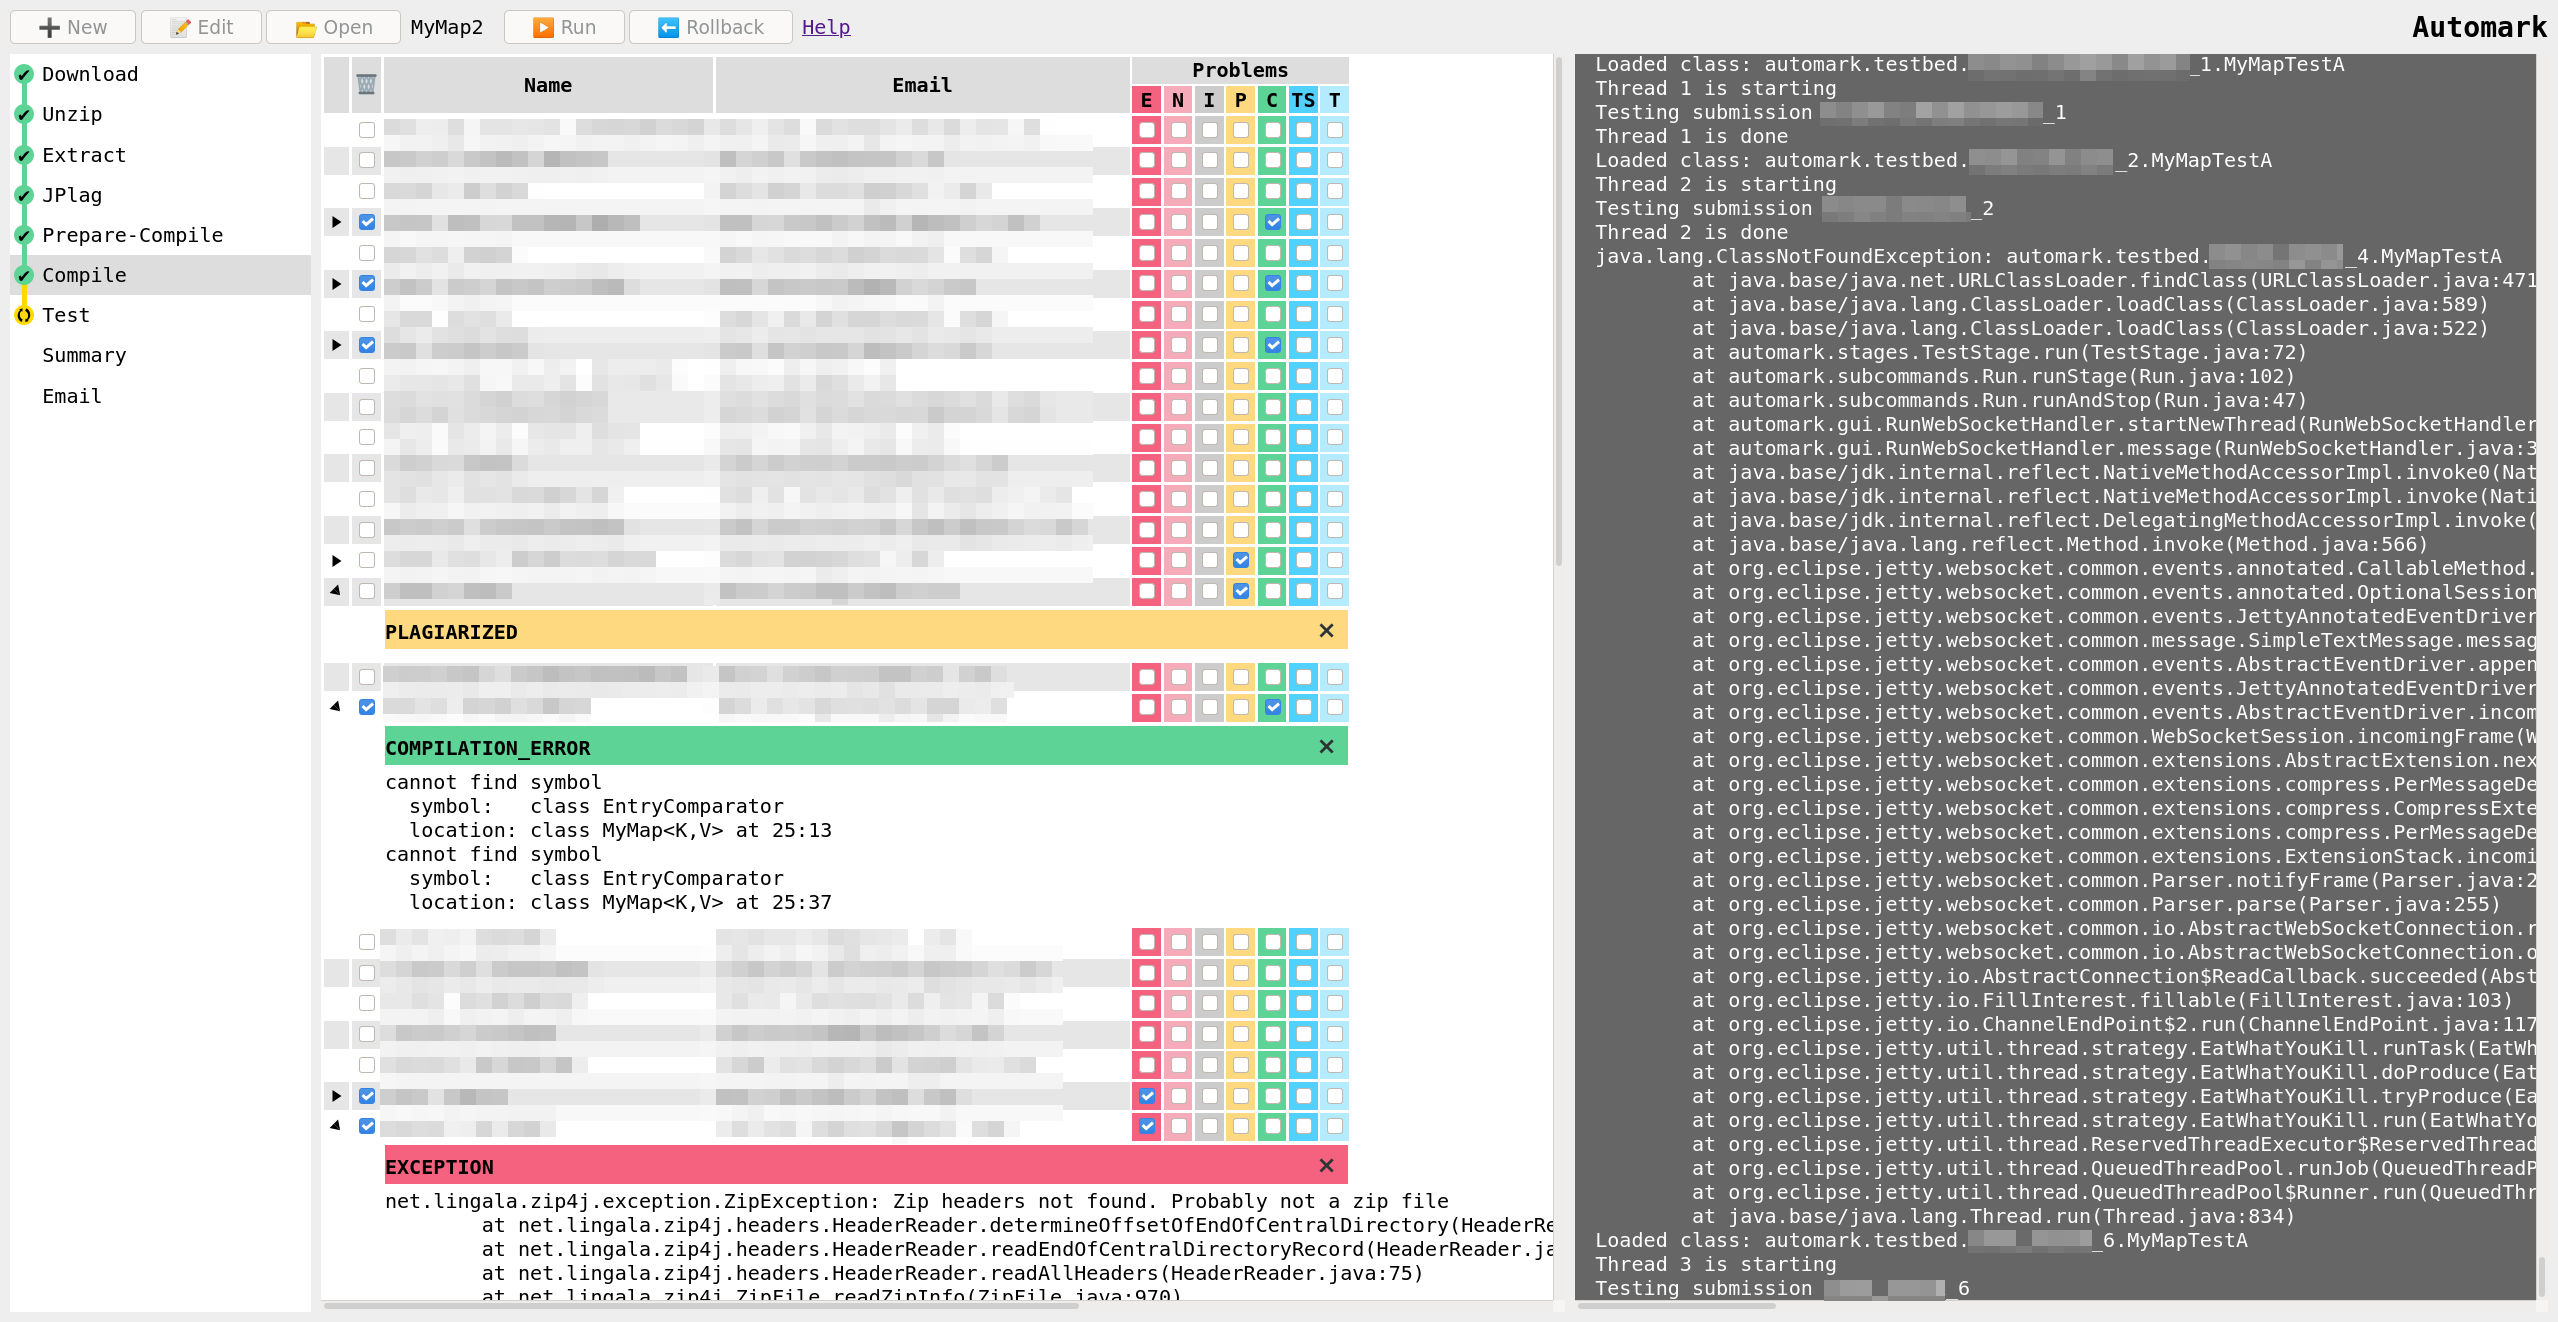
\includegraphics[width=10cm,trim=11.5cm 10cm 40cm 2cm,clip]{automark_dashboard_w_details_expanded.png}
		\caption{Automark submissions table}
	\end{figure}

	\subsubsection{Terminal Output}
	The rightmost panel on the Automark dashboard relays output that would have been printed to stdout when used over the CLI. Input is not handled by this panel but rather by pop-up windows, since implementing a web-based terminal emulator or even integrating an existing solution would have been out of scope for the Easy Mark One project.

	\begin{figure}[h]
		\centering
		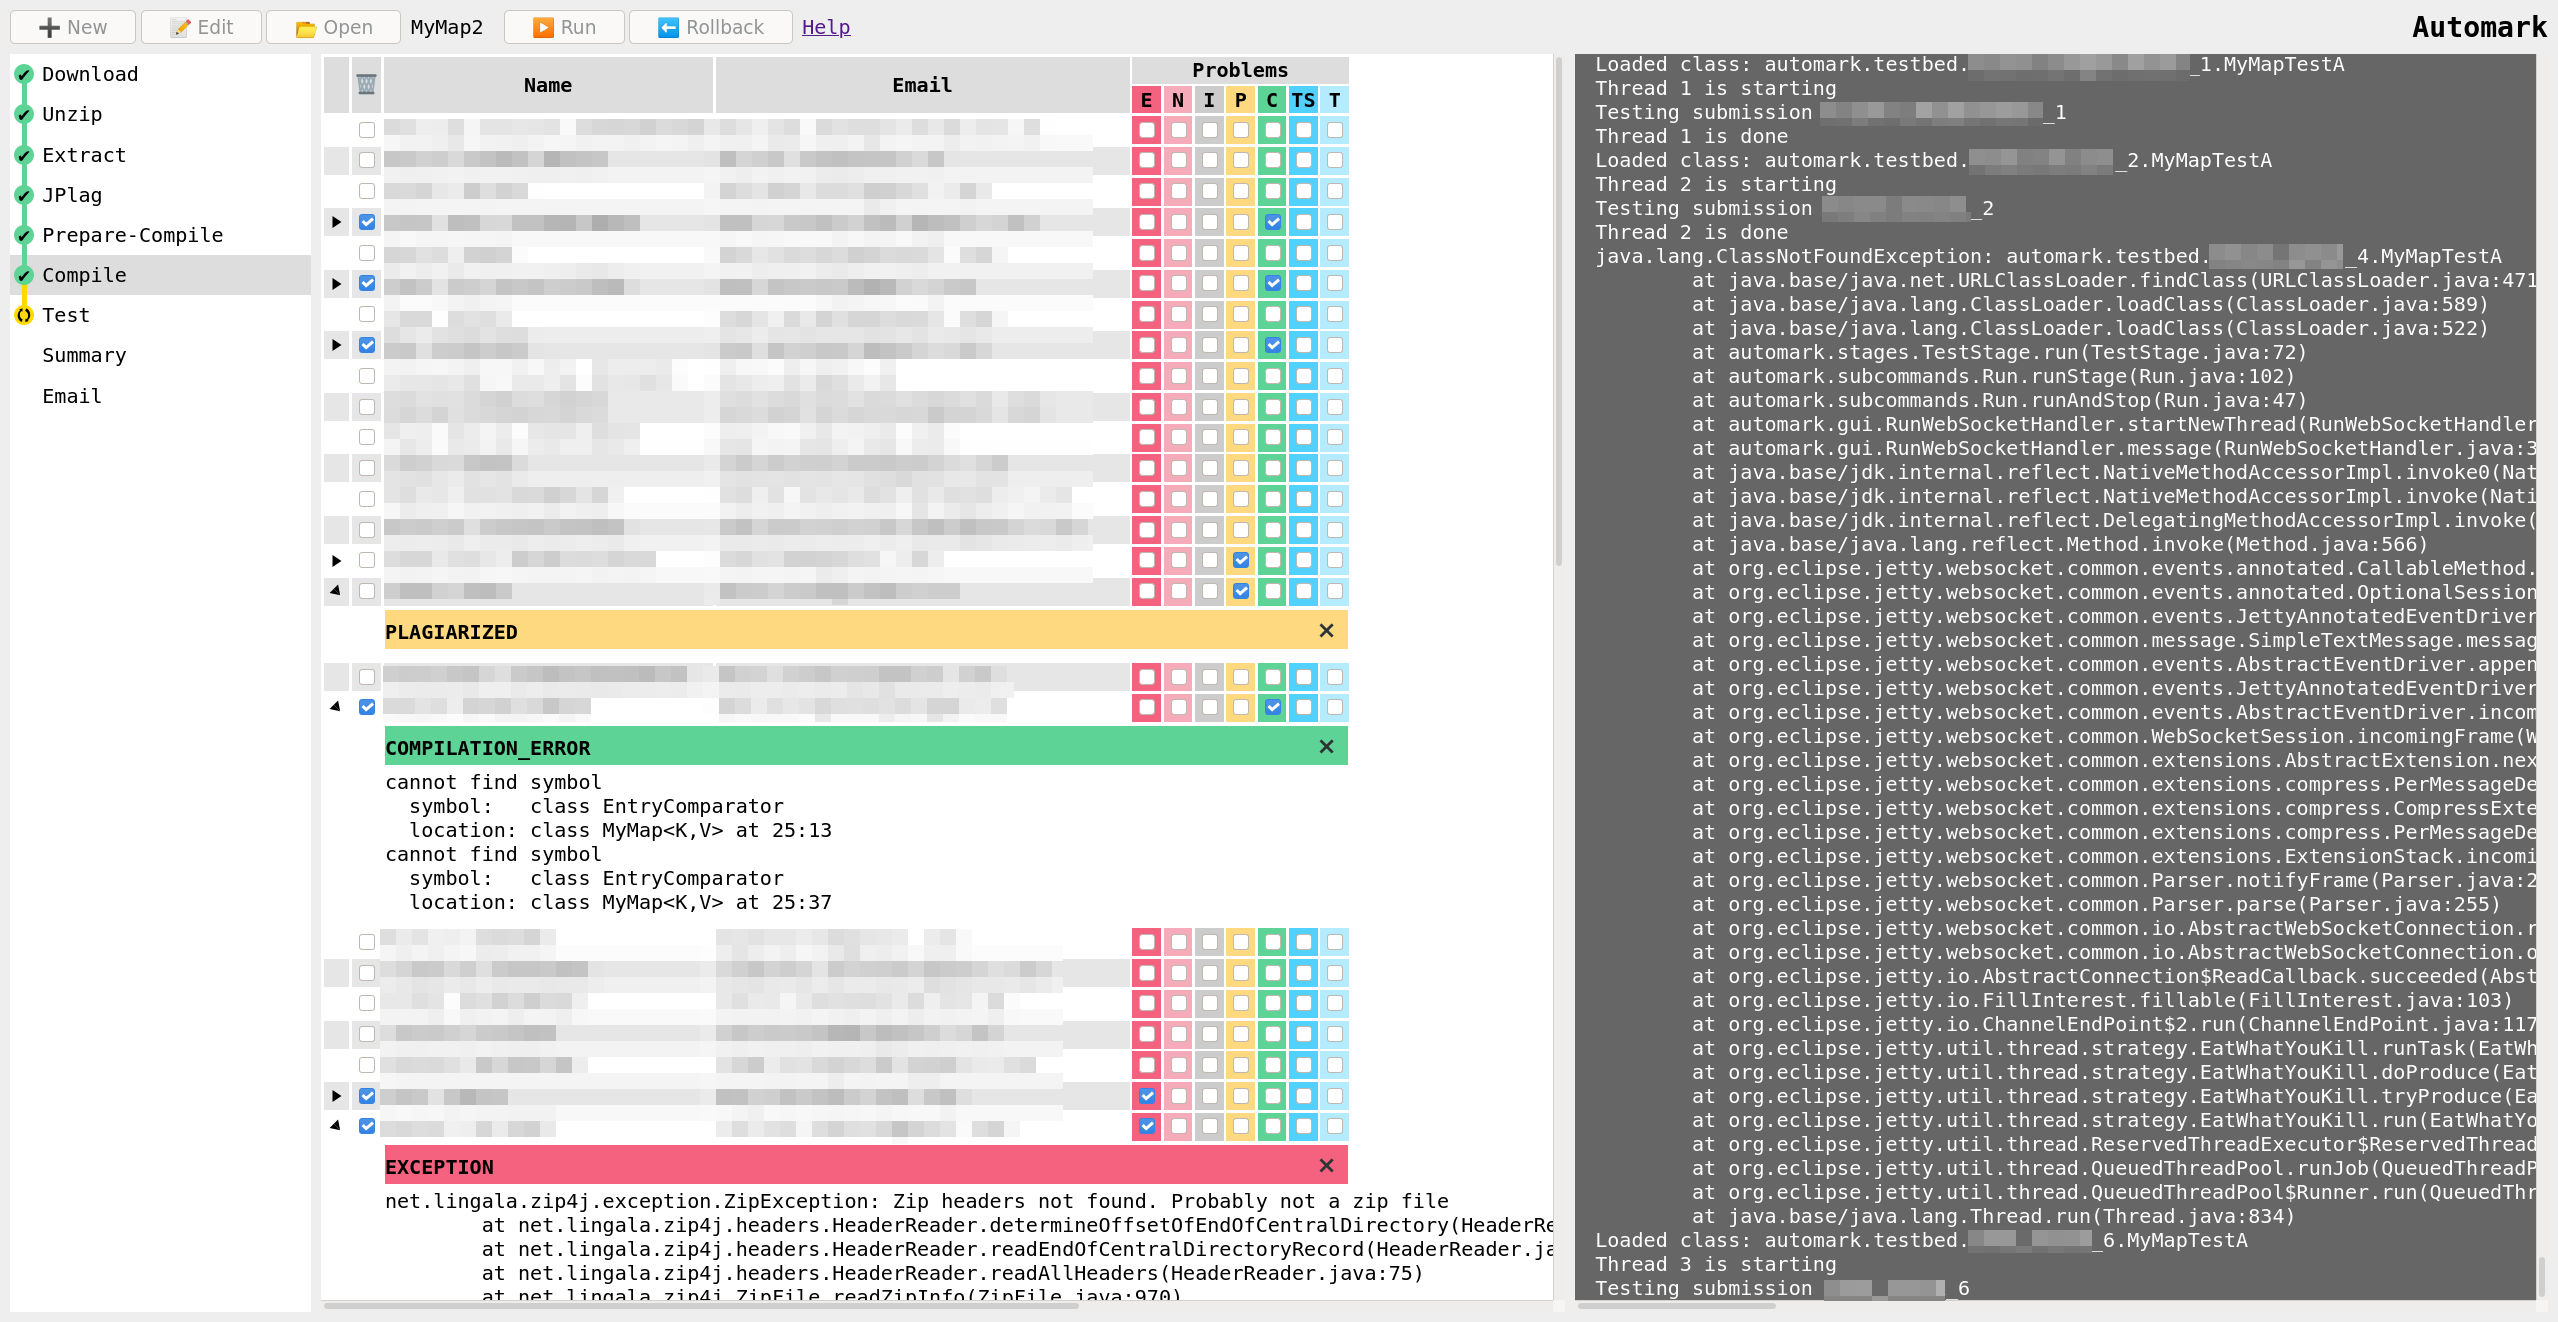
\includegraphics[width=10cm,trim=56cm 20cm 0 2cm,clip]{automark_dashboard_w_details_expanded.png}
		\caption{Automark terminal output panel}
	\end{figure}

	\subsubsection{Manual Page}
	Similarly to the CLI the GUI includes a formatted version of the manual page. it can be read by following the "Help" link on the dashboard. The manual page also describes in detail how GUI actions are related to CLI subcommands.

	\section{Internal Structure}

	\begin{wrapfigure}[16]{l}{.4\textwidth}
		\vskip-20pt
		%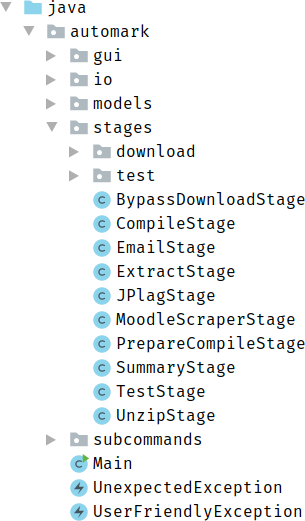
\includegraphics[width=.35\textwidth]{automark_code_structure.png}
		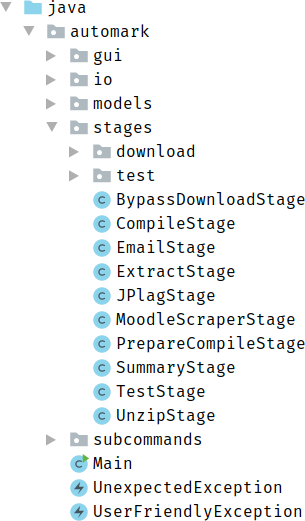
\includegraphics[width=.312\textwidth]{automark_code_structure.png}
		\caption{Automark's structure}
	\end{wrapfigure}

	Automark's code is divided by responsibility and grouped into accordingly named packages.

	It uses object-oriented programming (OOP) features very sparingly to avoid common OOP pitfalls like unnecessary or premature abstraction. Instead it relies mostly on static methods, switches and enum types and limits state to the method boundaries to facilitate a more procedural programming style.

	Stages are implemented as public static methods called "run" in the respective stage class and take the current working directory, the parsed config and the current submission metadata as their parameters. They are given full access to the file system but are expected to not modify the results from previous stages. Stage methods return an updated instance of the submission metadata (can be the same as the argument given to it). The returned metadata is then written to disk by the framework which marks the stage as completed. This design provides strong safety guarantees: If a stage crashes midway through, the metadata is never written and it is not regarded as completed.

	The GUI is implemented in JavaScript using Preact (see \ref{subsubsec:preact}~Preact). Action invocations are handled largely by preparing arguments for and calling subcommand methods (from within the program, not via the command line interface).

	\chapter{EasyMark}
	EasyMark is an online platform to connect students and teachers and share information about grades and assignments.

	\section{Technology Used}
	Just like Automark, EasyMark is implemented in Java which means the basic development tools are the same. This includes \ref{subsec:java}~Java, \ref{subsec:gradle}~Gradle and \ref{subsec:intellijidea}~IntelliJ~IDEA.

	\subsection{GSON}
	EasyMark stores its database in a JSON file, hence why it uses Google's GSON library. For more information about GSON and why it was chosen see \ref{subsubsec:gson}~GSON.

	\subsection{Javalin}
	Javalin is \emph{A simple web framework for Java and Kotlin}\parencite{javalinwebsite}. The majority of EasyMark's code consists of Javalin web resources. Javalin was chosen after several bad experiences with Spark in Automark (such as obscure rules for ordering declarations, hard-to-predict security features and having everything global by design). While Spark is still fine for the local use case in Automark, EasyMark is an internet-connected publicly accessible server, hence why a better framework was needed. Javalin and Spark also share a common ancestry with Javalin initially being a fork of Spark, however it later transitioned into a full rewrite.

	\subsection{Pebble}
	Pebble is a templating engine inspired by the Twig templating language\parencite{pebblewebsite}. It was chosen because it appeared to offer an above-average combination of usability and maintainance by the developers. Additionally, the author was already familiar with Twig from an earlier internship so less time had to be spent learning Pebble compared to other templating languages.

	\subsection{Spring Security}
	Spring Security is used for cryptographic functionality in EasyMark. This includes hashing of access tokens and symmetric encryption of sensitive information using up-to-date (and continuously updated) implementations of cryptographic algorithms\parencite{springsecuritywebsite}.

	\pagebreak
	Java provides cryptographic functionality in most JDK/JRE (Java Development Kit/Java Runtime Environment) distributions. However, the main concern with Java's builtin cryptography was that it is much less simplified than Spring Security's APIs, which in the case of cryptography, can lead to security issues by misuse of cryptographic mechanisms\parencite{javacryptographyusesinthewild}.

	Spring Security is used without the Spring web framework.

	\subsection{Hosted Instance}
	The hosted instance uses some additional technology to provide its services.

	\subsubsection{Google Compute Engine} \label{subsubsec:googlecomputeengine}
	Google Compute Engine (GCE) is the virtual machine product on the Google Cloud Platform (GCP)\parencite{gcewebsite}. It is used to host the production instance of EasyMark and was chosen because it provides a free tier which was estimated to be able to satisfy EasyMark's requirements.

	\subsubsection{Debian} \label{subsubsec:debian}
	Debian is a Linux-based operating system\parencite{aboutdebian} provided by default by the GCE. It was chosen because of its popularity, quality and support as well as the author's familiarity with it. The specific version used is Debian Buster (10).

	\subsubsection{Caddy} \label{subsubsec:caddy}
	\emph{Caddy 2 is a powerful, enterprise-ready, open source web server with automatic HTTPS written in Go}\parencite{caddywebsite}. It is used as a reverse proxy on the EasyMark instance and was chosen because of its simplicity of use and configuration as well as the author's familiarity with it.

	\section{Functionality}
	EasyMark provides an environment for teachers (referred to as "admins" by EasyMark) to create one or more courses and register student profiles for (referred to as "participants" by EasyMark).

	Participants are always bound to one course. If a student participates in two courses there will be two participants in the database. The participant's name (which is the only directly personally identifiable information in the system) is encrypted with the access token of the admin who created it. This means the participant isn't able to see their own name on the site but it also means bad actors that were able to obtain information from the database will not be able to see the names either.

	A course can have assignments divided into chapters. Chapters can optionally contain a special "test" assignment to which participants can volunteer after completing the assignments in the chapter (which by EasyMark is referred to as "sending a test request" or "requesting a test").

	\pagebreak
	Admins have a built-in editor for managing participants' grades. The editor is built like a spreadsheet and enables admins to enter the score reached by a participant for any assignment. Assignments are created with a maximum score although the teacher is able to give a higher score than the maximum if that is nedded.

	\subsection{Zones}
	Pages on the EasyMark site are divided into "zones" i.e. areas that are only accessible to users with certain roles. There are three zones in EasyMark: The \textbf{public} zone which includes the login page as well as static assets such as CSS and JavaScript scripts, the \textbf{participant} zone which includes the public zone, a view of the participant's progress in their course and the ability to send test requests and the \textbf{admin} zone which includes the public zone, the admin dashboard with the ability to create courses and delete test request, the course editor with the ability to create, delete and edit courses, chapters and assignments and the grading editor with the abilty to create and delete participants and edit participants' scores. Lastly the settings pages is also part of the admin zone with the ability to create and delete other admins, reset their access token and backup and restore information that would be encrypted on the server in unencrypted form.

	\subsection{Access Tokens} \label{subsec:accesstokens}
	Access tokens (sometimes shortened to "AT") are 48-character long hexadecimal strings. That means they can only consist of the numbers zero to nine and the caracters "a" to "f". Access tokens are generated by the server and randomized.

	The reason for using access tokens instead of a classic username/password authentication scheme was that usernames were an unnecessary complication and possible data protection liability if they were derived from personally identifiable information such as the name and user-chosen passwords would be less secure than randomized ones on average. Technically, access token authentication as employed by EasyMark boils down to username/password authentication but with fully randomized usernames and passwords.

	Since users do not have anything like a username, the first eight characters of an access token are stored in clear in the database and used for identification of the user. The reason for this is that the hash function used to process the password for verification is intentionally slow so that it takes bad actors who have obtained password hashes from the database  longer to brute force them. Therefore it would not be feasible, even with only a few users, to identifiy users by hashing the provided access token again and again and comparing it to the hash in the database.

	Hashing the password once and comparing it multiple times is not easily possible since Spring Security automatically appends random characters (called a "salt") before hashing text which it then stores alongside the hash. This is normally a security measure for user-chosen passwords to prevent so-called "rainbow table attacks" where a bad actor pre-hashes common passwords and compares only the hashes as well as well as having similar hashes for similar passwords in the database. For EasyMark it would theoretically not be necessary to salt access tokens since access tokens are always long randomized strings but due to security considerations it has been decided that it is better for the project to use Spring Security as-is and not try to circumvent it.

	Access tokens are only displayed once on the admin's screen who created the user. The admin is asked to copy or share the access token immediately since it will never be displayed again. The server at that point does not have access to the raw access token anymore.

	Access tokens of participants are referred to as "course access tokens" or "CATs" for short throughout the EasyMark UI and code to differentiate them from admin access tokens. Technically there is no difference between a CAT and an admin AT.

	\subsection{Sessions}
	Sessions are the association of multiple page views and data such as authorization roles with one another based on authentication. Sessions typically start with a login and end with a logout and are tied to one browser and device. Sessions are necessary to implement zones and users.

	To implement sessions EasyMark makes use of a feature provided by the Javalin framework which automatically sets a session cookie with a framework-generated session ID in the client (the browser). This cookie is then used to re-identify the session. Javalin provides a map (a key-value data structure) to the application which it can use to store session data. EasyMark, when creating a session, manages sessions itself in a seperate session manager. It only stores a reference to the session in the session manager in Javalin's session map. This reference is a UUID (universally unique identifier).

	When logging in, after verifying the user's access token a session is created and registered and the provided access token is discareded again. It is not used anymore until the next login. This brings the benefit of making sessions revokable over another session. Especially in EasyMark's context this is useful since students or teachers might log in over a stationary computer at school and forget to log out afterwards.

	Sessions expire after five hours of inactivity.

	\subsection{Database}
	EasyMark uses a JSON file as its database. The reason for this decision was that database access frameworks and libraries available in the Java ecosystem where deemed too complicated to learn and implement in the project's limited time span.

	The model behind the JSON file is designed like a relational database schema: The root object includes lists of entities with UUIDs as primary keys and references to other entities are stored as UUIDs. The only exception to this design are access tokens which are stored as JSON objects with the identifier and secret parts as properties.

	See \RefAppendix{A} for the database schema.

	\section{User Interface}
	Being an internet-connected multi-user web application EasyMark is mostly used over a web browser. However, for some administrative tasks EasyMark provides a command line interface.

	\subsection{Command-Line Interface}
	EasyMark provides a command-line interface for creating and deleting admins as well as resetting admins' access tokens. This was implemented as a "last-resort" option if, for example, all admins have forgotten their access tokens. For that case it was chosen access to the server counts as a proof of authenticity for an admin. Classic solutions to this problem like using email as a proof of authenticity would have taken too long to implement and would have posed additional security and data protection problems. Note that access to the command line interface or the server does not grant access to encrypted data.

	Like the Automark CLI, EasyMark's interface is divided into several subcommands. These are the subcommands provided by EasyMark:

	\begin{description}
		\item[serve] Starts the web server on port 8080

		This is also the default subcommand when no subcommand is specified.

		\textbf{Syntax:}\tabto{75pt}\lstinline|easymark [serve [--enable-insecure-debug-mechanisms]]|\\
		\textbf{Arguments:}\tabto{75pt}The \lstinline|--enable-insecure-debug-mechanisms| flag is only for development, testing or evaluation and \textbf{should not be used in production.} It indicates that the server should drop some security features and, among others, enable a feature by which users can bypass authentication by appending \lstinline[mathescape]!?debugChangeLogin=<admin|participant>! to URLs to gain any role they want. This flag should never be used on a production server or database, not even temporarily. It is only for local use.

		\item[create-admin] Creates a new admin account and outputs its access token

		It is recommended the operator stops the server while executing this command.

		\textbf{Syntax:}\tabto{75pt}\lstinline|easymark create-admin|

		\item[reset-admin-token] Regenerates an admin account's access token and outputs the new access token

		It is recommended the operator stops the server while executing this command.

		\textbf{Syntax:}\tabto{75pt}\lstinline|easymark reset-admin-token <admin-selector>|\\
		\textbf{Arguments:}\tabto{75pt}\lstinline|<admin-selector>| is either the ID (a UUID) of the admin to reset the access token of or the name of a course that admin administers

		\item[delete-admin] Deletes an admin account and all associated courses participants, chapters, test requests, assignments and assignment results

		It is recommended the operator stops the server while executing this command.

		\textbf{Syntax:}\tabto{75pt}\lstinline|easymark delete-admin <admin-selector>|\\
		\textbf{Arguments:}\tabto{75pt}\lstinline|<admin-selector>| is either the ID (a UUID) of the admin to delete or the name of a course that admin administers

		\pagebreak
		\item[debug-seed-database] Truncates the database and fills it with demo data used for debugging, development and testing

		Everything in that dataset is deterministic including UUIDs which means it can be (and is) used for testing.

		\textbf{A database generated by this command should never be used in production. Access tokens in the underlying dataset are public.}

		\textbf{Syntax:}\tabto{75pt}\lstinline|easymark debug-seed-database|
	\end{description}

	\subsection{GUI}
	The GUI makes up most of EasyMark's user interface. It is used over the internet in a web browser. Most of the GUI is simple and self-explanatory so not every page on the site is mentioned in this paper.

	\subsubsection{Login Page}
	A plain white page with a single input field in the center labelled "Access Token".

	\subsubsection{Participant Dashboard}
	\begin{figure}[H]
		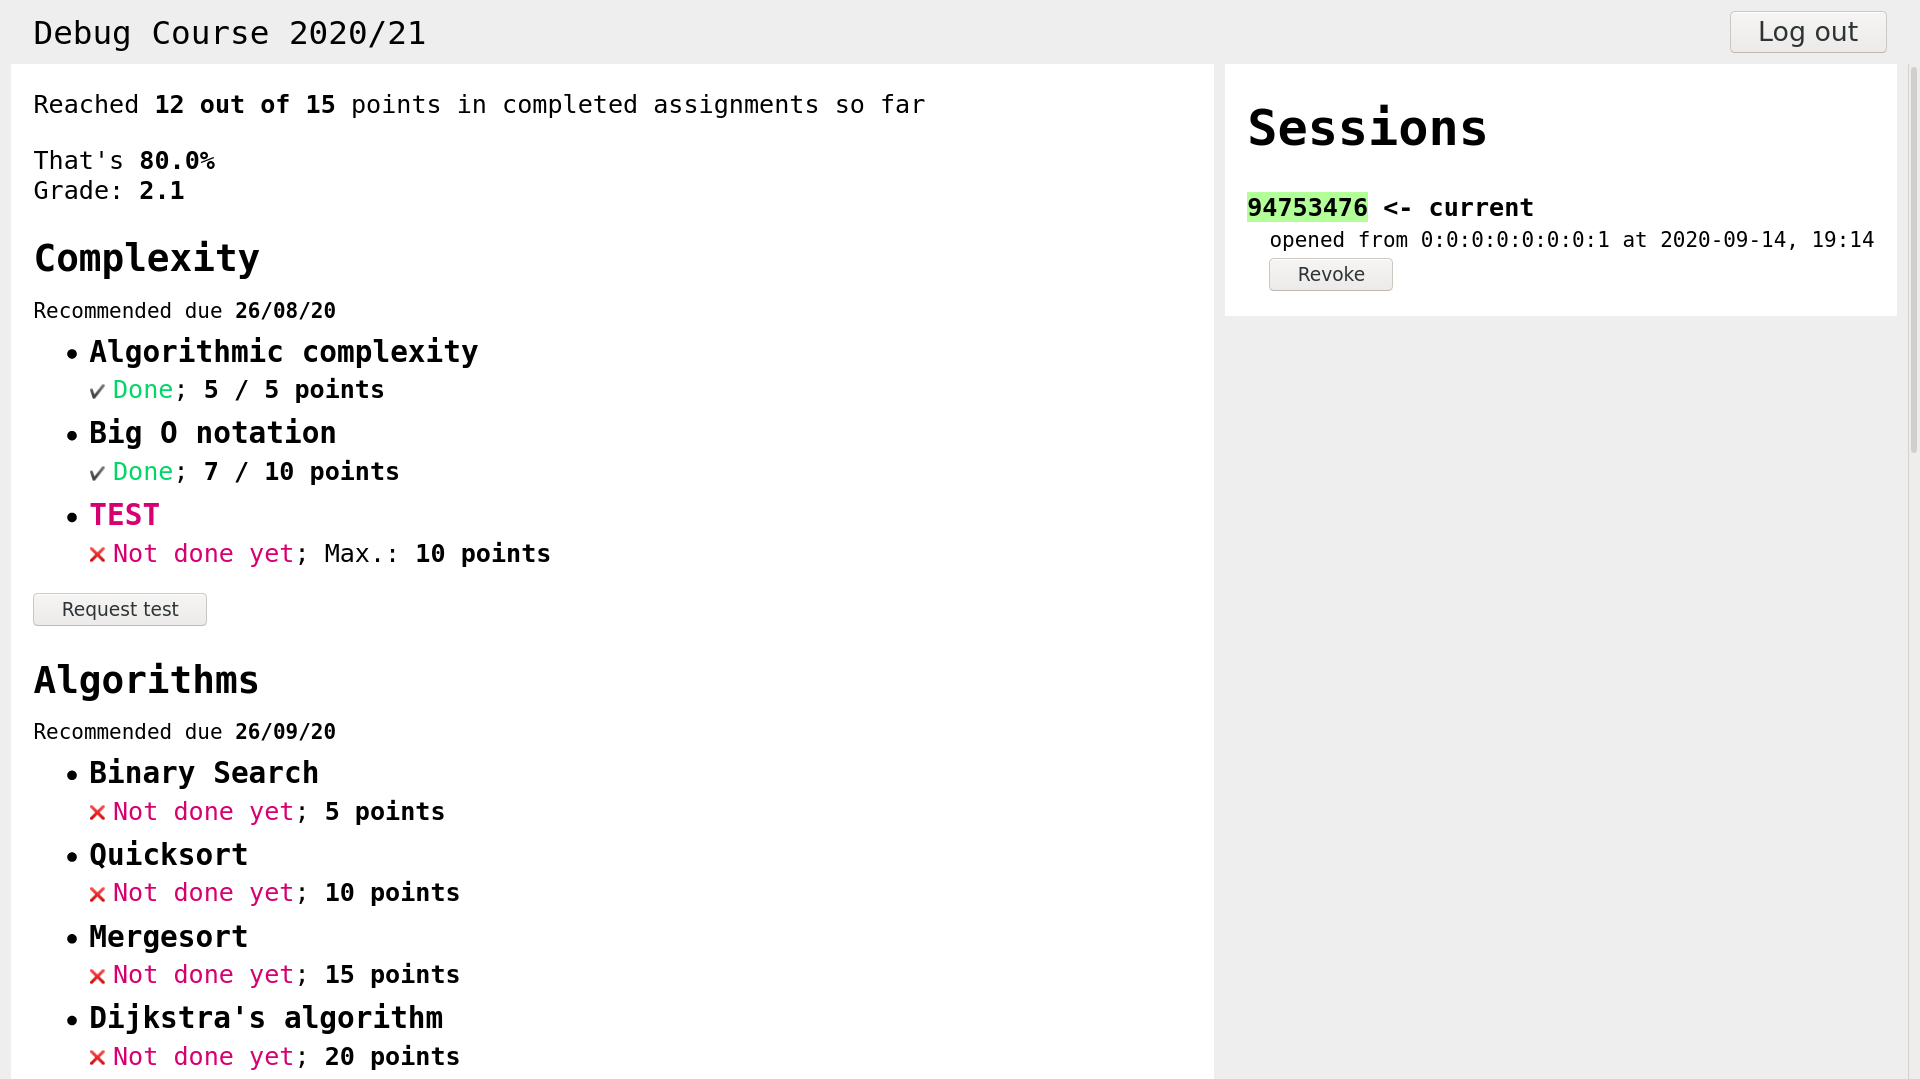
\includegraphics[width=\textwidth]{easymark_participant_dashboard.png}
		\vskip0pt
		\caption{Screenshot of the participant dashboard}
	\end{figure}
	The participant dashboard is what participants see when they log in.

	It shows the status of submissions, grades and active sessions with the ability to revoke sessions and request tests.

	\pagebreak
	\subsubsection{Admin Dashboard}
	\begin{figure}[H]
		\centering
		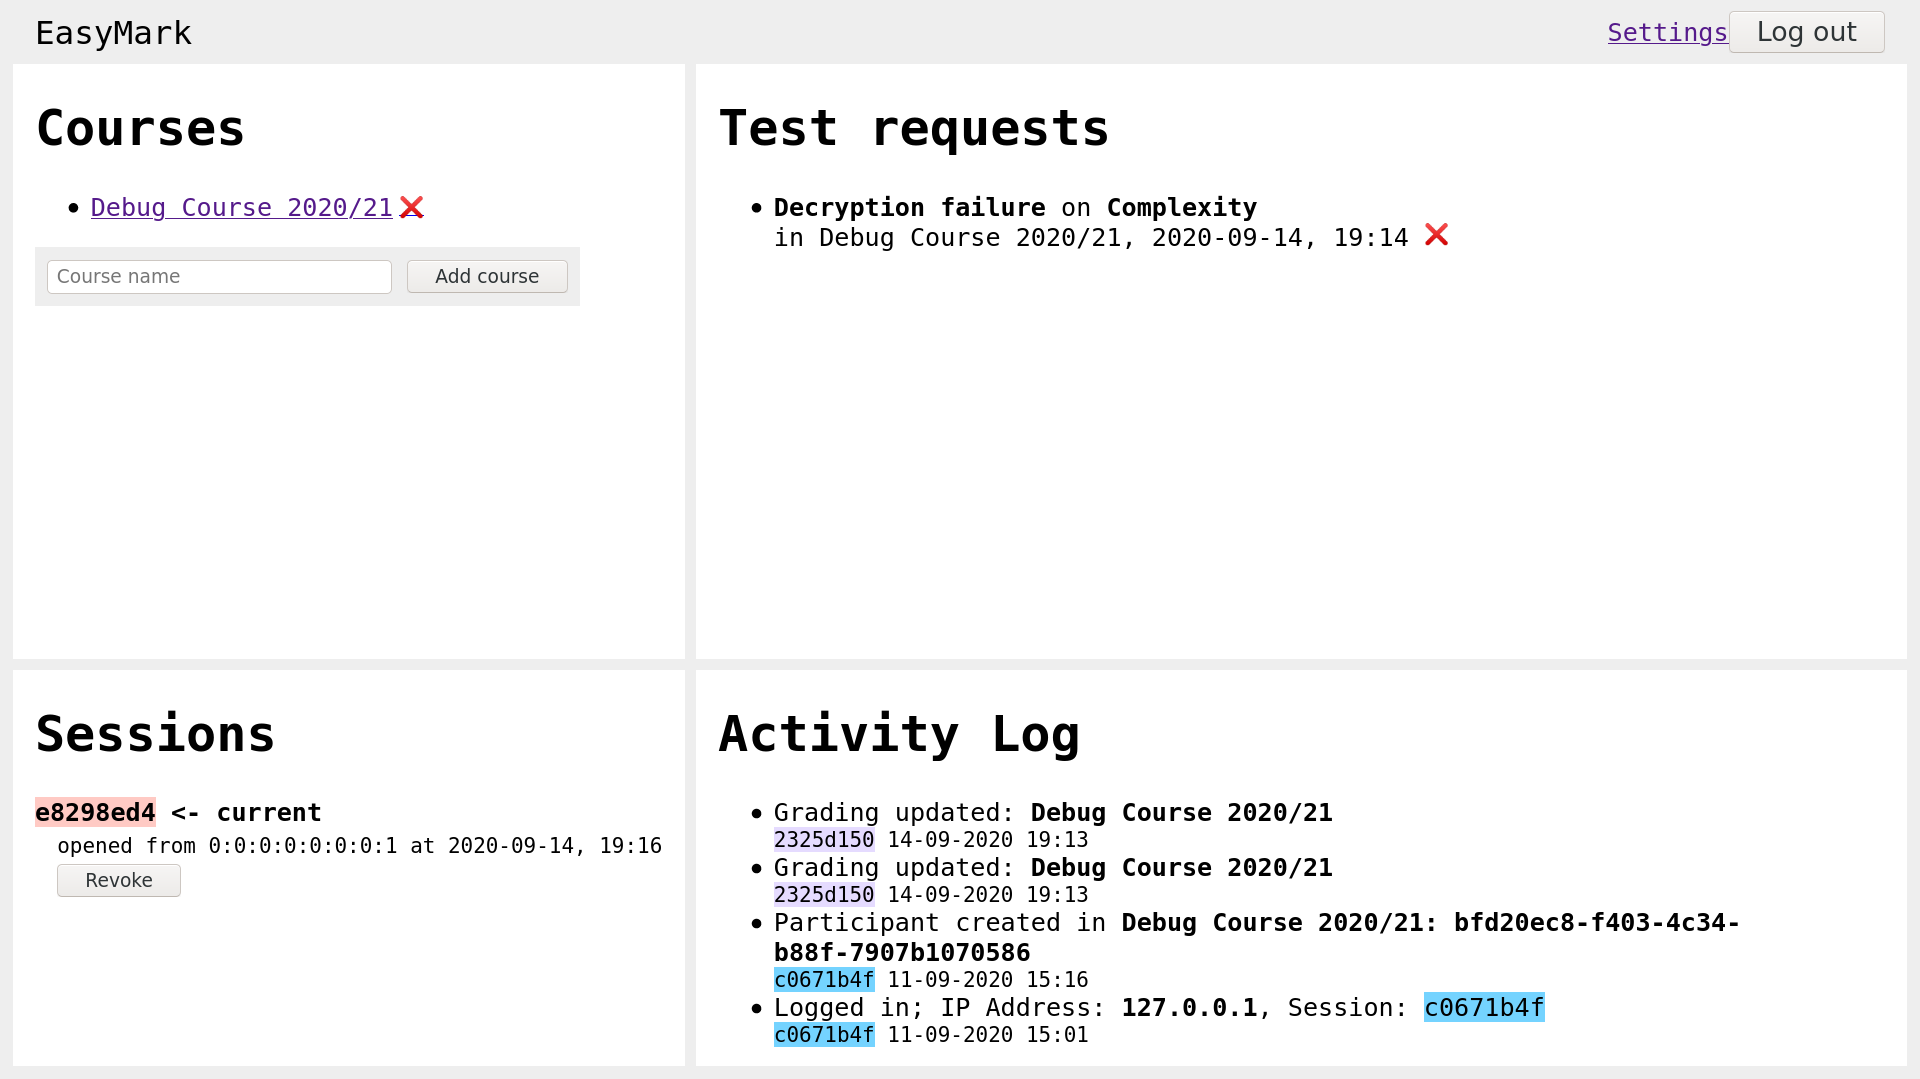
\includegraphics[width=.95\textwidth]{easymark_admin_dashboard.png}
	\end{figure}

	The admin dashboard is what admins see when they log in.

	It lists courses and links to the course editor, lets the admin create and delete courses and test requests from the top two panels.

	At the bottom there are panels to monitor account activity and sessions and revoke sessions remotely. This is the same session manager component as on the participant dashboard.

	\subsubsection{Course Editor}
	The course editor is used to edit the structure of a course. That includes creating, editing and deletign chapters and assignments, editing and deleting the course itself.

	\begin{figure}[H]
		\centering
		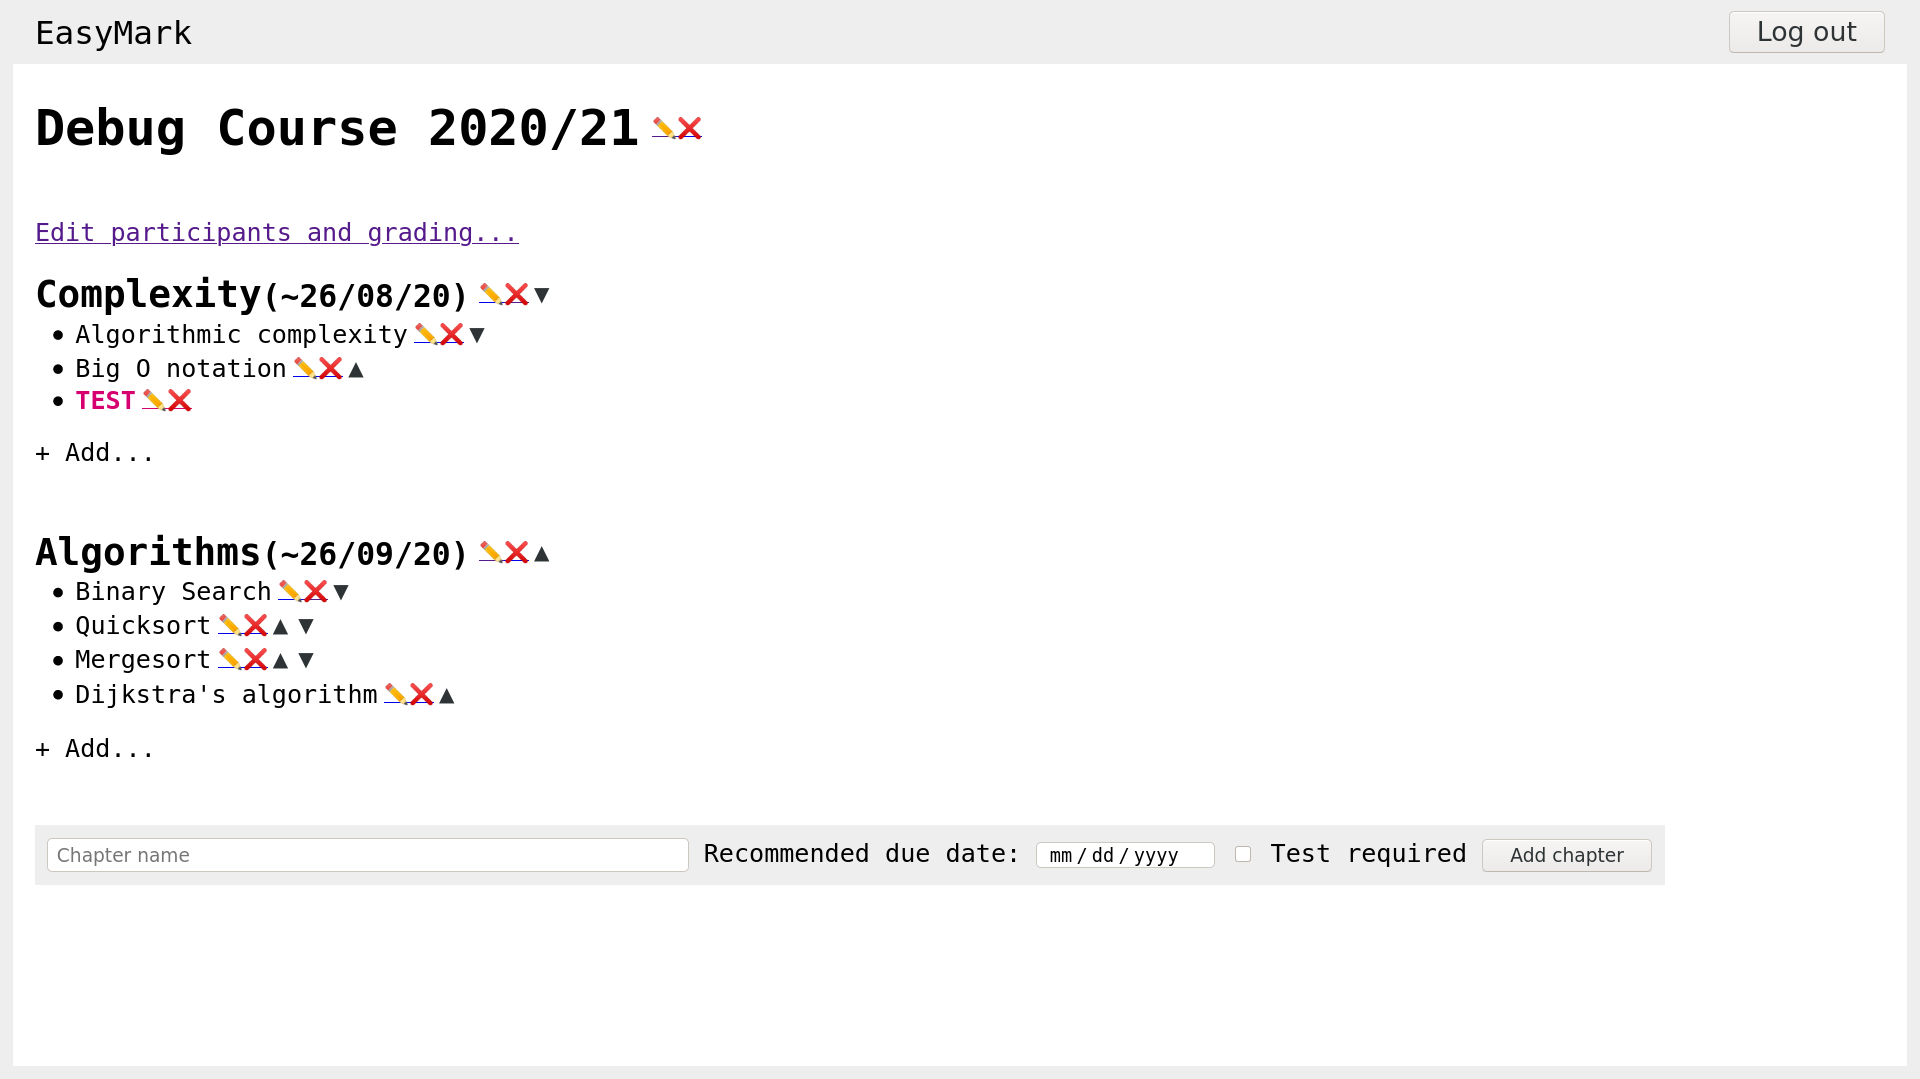
\includegraphics[width={.95\textwidth}]{easymark_course_editor.png}
	\end{figure}

	\subsubsection{Grading Editor}
	The grading editor is used to enter participants' scores on completed assignments as well as add, edit and delete participants.

	It is used and structured like a spreadsheet with participant names as the row keys and assignment names grouped by chapters used as column keys. there are also a few special columns before the assignment columns to reset a participant's course access token, record additional administrative data not shown to the participant and see participants' grades.

	\begin{figure}[h]
		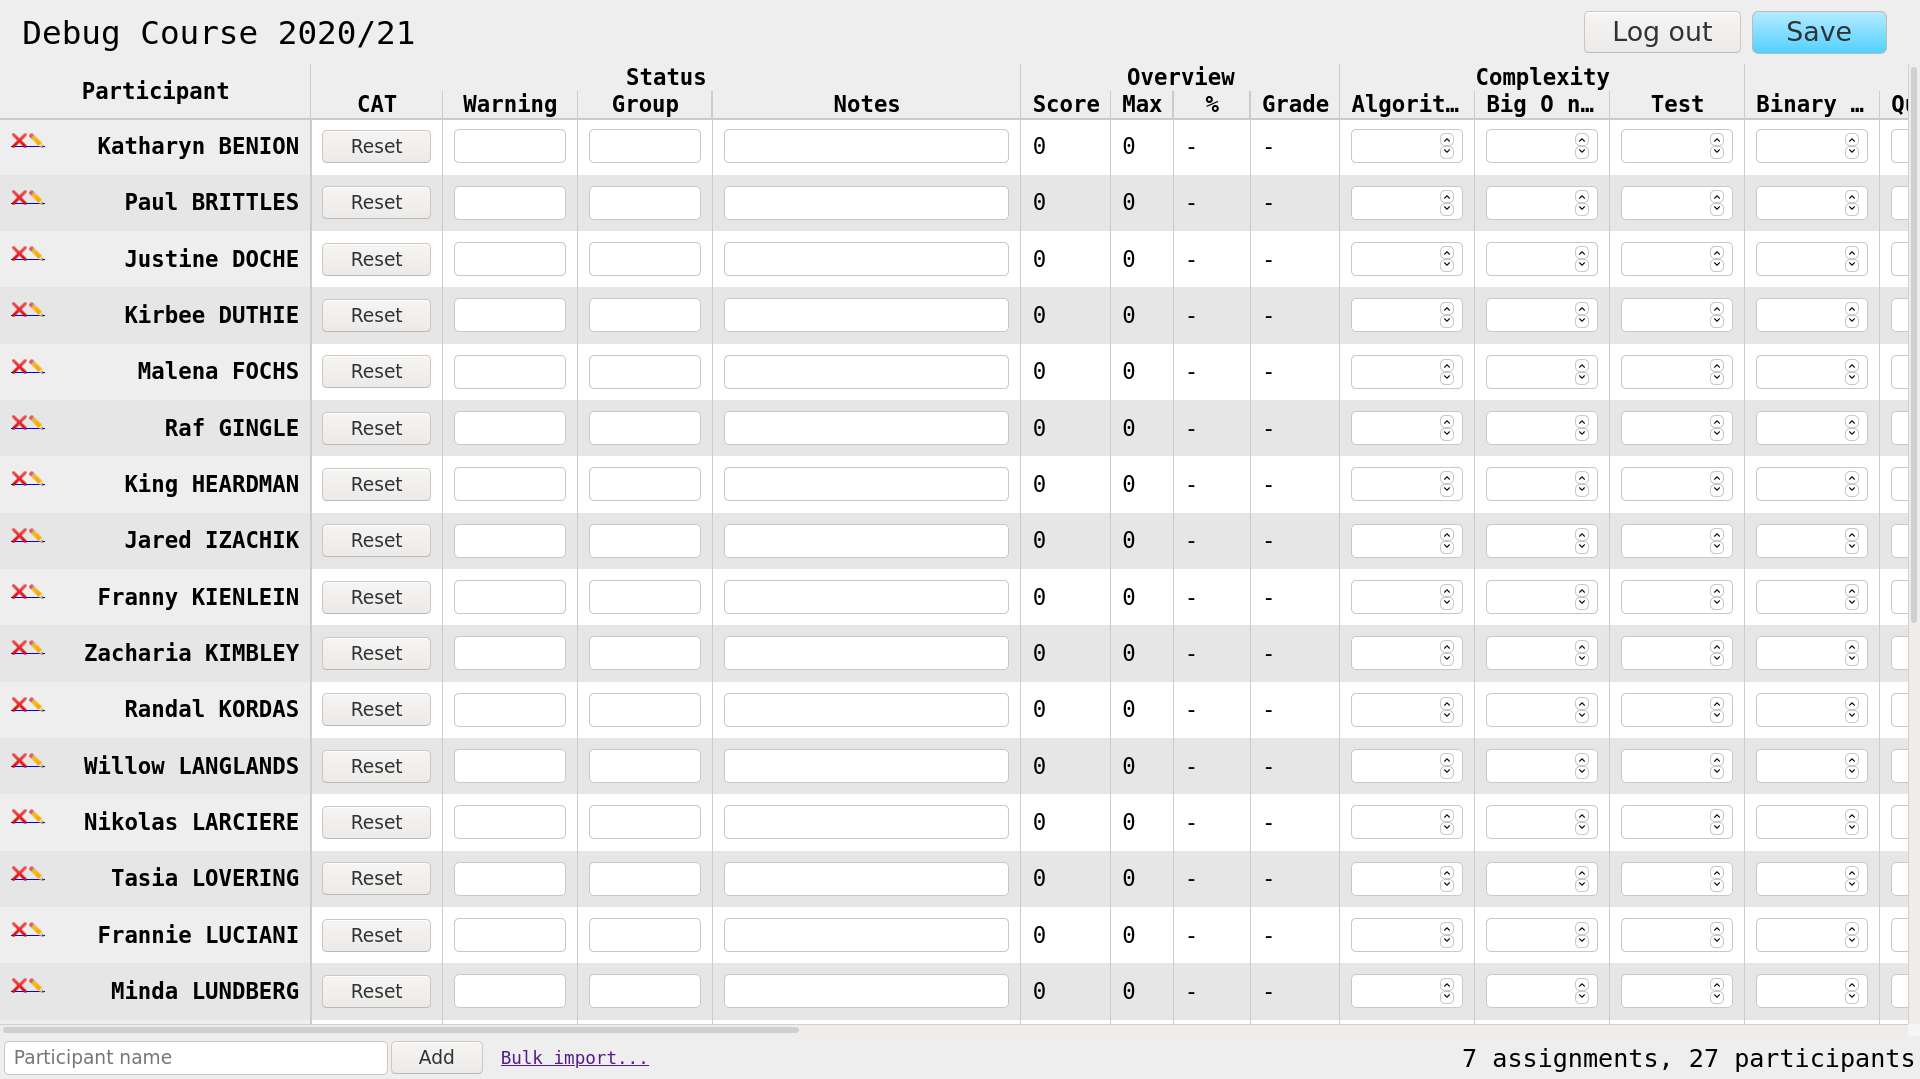
\includegraphics[width=\textwidth]{easymark_grading_editor.png}
		\vskip0pt
		\caption{Screenshot of the grading editor with the debug dataset}
	\end{figure}

	When scrolling, the name column is fixed to the left. The table header with the column keys and group names is fixed to the top. The topmost and bottommost toolbars are fixed in-place entirely.

	\subsubsection{Settings Page}
	\begin{wrapfigure}[13]{l}{.55\textwidth}
		\vskip-15pt
		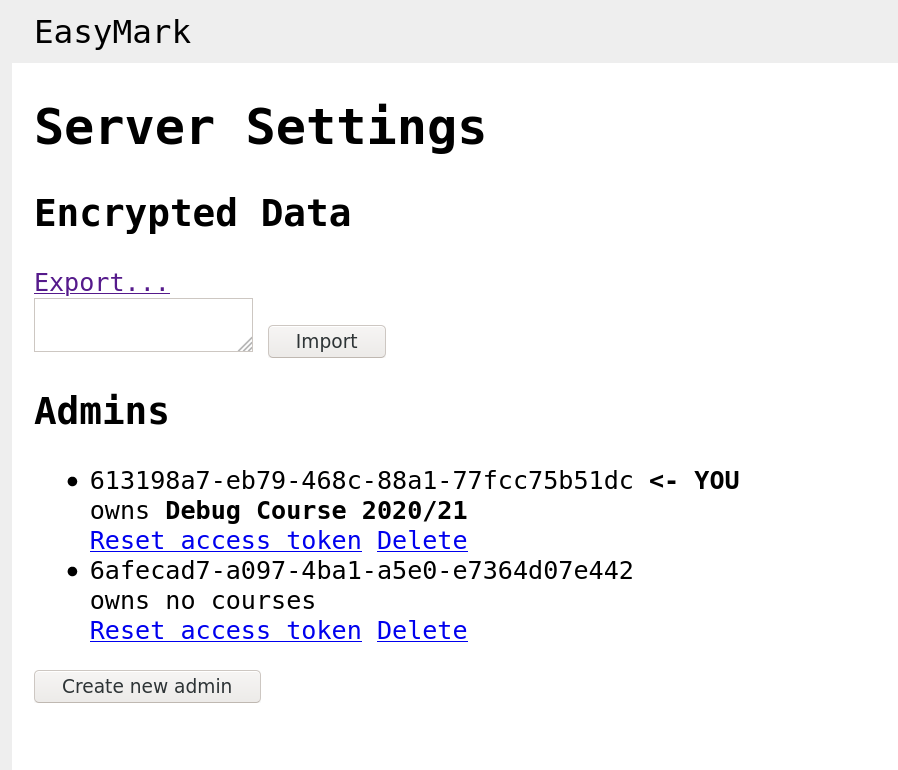
\includegraphics[width=.55\textwidth,trim=0 1cm 0 0,clip]{easymark_settings.png}
	\end{wrapfigure}

	The settings page gives admins the ability to export and re-import encrypted data for their account, for backup purposes. This is especially useful when an admin forgets their access token and has to have it reset, since encrypted data associated with that admin on the server is unrecoverable after an AT reset.

	Located below that are controls to create, delete and reset the access tokens of admins. Every admin can reset the access token of or delete not only their own account but also the account of every other admin, so only trusted people should have access to an admin account.

	When resetting the access token of an admin, one can optionally provide the old access token. If provided, the server will use it to decrypt and re-encrypt encrypted data associated with that admin with the new access token so that the data remains accessible.

	\section{Security}
	This chapter details the security measures taken in EasyMark and gives reasoning for decisions and considerations on security measures.

	\subsection{Access Tokens and Access Token Verification}
	As mentioned in \ref{subsec:accesstokens}~Access~Tokens, access tokens are 48 character long random hexadecimal strings, eight of which are stored in clear in the database and used for finding the user (admin or participant) account the client claims to be. The remaining 40 characters are used to verify that the client is authorized to access the account (i.e. as a password).

	Access tokens are only ever generated by the server and are only displayed once in the UI. The secret part (the last 40 characters) of an access token is run through a cryptographic hash function before being stored in the database. The specific hash function used is bcrypt implemented by Spring Security as the \lstinline|BCryptPasswordEncoder|.

	When a user logs in, EasyMark first finds the appropriate account via the identifier part (the first 8 characters) of the access token provided. Then, if it has found one, it hands the secret part (the last 40 characters) of the access token and the hash from the database to Spring Security which verifies that the provided string matches the hash (including any security measures added on top internally such as salting).

	\subsection{Personally Identifiable Information}
	Data that directly identifies the person behind a participant account is classified as personally identifiable information (PII) and symmetrically encrypted using an encryption mechanism that makes it ultimately accessible using the access token (all 48 characters) of the admin that owns the course the participant is registered in. This also means that the participant is not able to view their own PII. To comply with regulations admins might have to disclose this information to participant account holders on request.

	Currently, only the participants' names are classified as PII. Other PII commonly stored by online platforms such as email addresses are not collected by EasyMark.

	The information is not directly encrypted with the admin's access token. This would mean that the access token must be stored in clear somewhere where it is associated with the session. On the server this would be undesirable since it might entail security disbenefits to handle access tokens in cleartext over extended periods of time. On the client this would be undesirable since it would make sessions un-revokable in practice if the access token is just visible in one of the browser's storage mechanisms.

	Instead, upon registration of an admin a seperate encryption key is generated called the "user encryption key" (UEK). This is the key used to symmetrically encrypt sensitive information. The key is then encrypted with the access token of the new admin (which the server has because it has just been generated). The UEK encrypted with the access token forms the so-called "initial encryption key" (IEK) for the new admin. The IEK is stored in the database next to the access token identifier and hashed secret part. The UEK and raw access token are discarded and handled by Java's garbage collection.

	When an admin now logs in, their supplied access token is used to decrypt the IEK from the database (after all other login checks) to obtain the UEK. Then, another enryption key is generated called the "session encryption token" (SET). The SET is used to encrypt the UEK, which forms the so-called "session encryption key" (SEK). The SEK is stored in the admin's session in the session manager, the SET is sent to the client to be stored as a session cookie (alongside the session ID cookie).

	When an admin performs a request for which the server needs to decrypt sensitive information, the server takes the SET (which it has because the client sent it as a cookie with the request) and the SEK (from the session store) and decrypt the SEK to obtain the UEK. It can then decrypt sensitive data from the database with the UEK and send it to the client. the SET and the UEK are thrown away after the request and handled by Java's garbage collection.

	\begin{figure}[H]
		\centering
		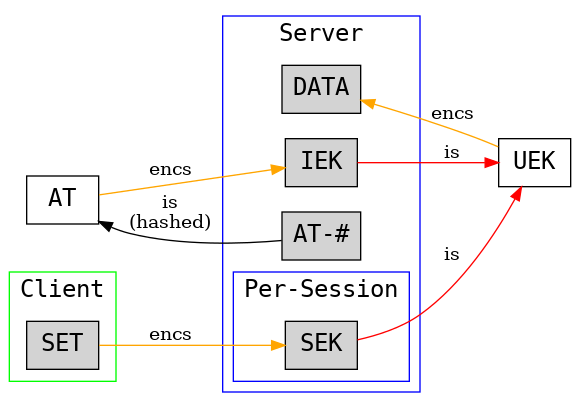
\includegraphics[width=.7\textwidth]{easymark_encryption.png}
		\vskip0pt
		\caption{Diagram showing the different components of EasyMark's encryption}
	\end{figure}

	This scheme has the benefit of allowing sessions to be revoked. If the server wants to revoke a session (either after a timeout or on the admin's behalf) it simply throws away the SEK together with the session in the session manager. The client might still have the SET but the SET alone is useless.

	The server can also not decrypt information entirely on its own since it needs a request from the client with the SET first. Although if bad actors are able to hijack the server and intercept requests or view the server process's memory, they are able to decrypt sensitive information.

	End-to-end encryption would prevent that but end-to-end encryption poses challenges for revokability. A seperate "encryption token" could be used only for admins similarly to the access token but it is only used for encryption and never sent to the server. The drawback of this approach would be that the key can't be taken away from clients that are not in control of the admin (like a stationary school computer). That means that a bad actor who has access to such a client and the database contents could decrypt sensitive information. It should be noted that both this scenario and the scenario of bad actors hijacking or replacing the server's process were deemed unlikely.

	The encryption algorithm used for sensitive data (PII) is 256 bit AES in the Galois/Counter Mode of operation. It is implemented in Spring Security via the "delux" encryptor\parencite{springdocssecurityencryptors}.

	\subsection{CSRF Protection} \label{subsec:csrfprotection}
	\BlockCite{
		Cross-Site Request Forgery (CSRF) is a type of attack that occurs when a malicious web site, email, blog, instant message, or program causes a user's web browser to perform an unwanted action on a trusted site when the user is authenticated.

		A CSRF attack works because browser requests automatically include all cookies including session cookies. Therefore, if the user is authenticated to the site, the site cannot distinguish between legitimate requests and forged requests.
	}{owaspcsrfcheatsheet}

	EasyMark's underlying web framework, Javalin, does not provide out-of-the-box CSRF mitigation. Therefore, EasyMark implements the synchronizer token pattern. If a page that's about to be sent to a client (regardless of authentication) contains the ability for the user to do something that should be protected against CSRF (generally state-changing form submissions), the server generates a random CSRF token. CSRF tokens are randomized numbers of the Java data type \lstinline|long| converted to a string in decimal notation. CSRF tokens are stored in Javalin's session map. If they were stored in EasyMark's session manager it would be impossible to protect the login page since EasyMark only registers sessions for authenticated users in the session manager.

	If a request for a CSRF-protected route comes in EasyMark compares the provided CSRF token to the tokens associated with the current session in the session map. If one matches, EasyMark continues with the request and invalidates the token. If not, the request is denied.

	Multiple CSRF tokens can be valid at the same time to allow the user to have multiple tabs with protected actions open at the same time.

	CSRF tokens expire after 5 hours, regardless of session activity.

	Pages with CSRF tokens on them will also explicitly ask the browser not to be cached so that the functionality of history navigation (back/forward buttons) is not broken.

	\subsection{Caching}
	To prevent leakage of sensitive data some pages (like the pages that display access tokens after account creation) send the "Cache-Control" header with the value "no-store" to ask the browser not to cache them. Caching pages with sensitive information would risk showing that information to unauthorized parties which especially is a problem in EasyMark's case since EasyMark might be used from public computers (like stationary school computers).

	Pages with CSRF tokens on them also disable caching. See \ref{subsec:csrfprotection}~CSRF~Protection.

	\section{Deployment}
	Being a web application with a backend, EasyMark requires a host to run on. Additionally Easymark requires some extra infrastructure such as a reverse proxy in production environments. To accomplish this, a small framework has been written to automatically configure a virtual machine on the Google Compute Engine. The GCE-specific parts of the framework are small so it could also be ported to different environments. It is somewhat dependent on Debian as the host operating system although that can also be changed if needed.

	The framework is written in Bash and allows operators to write simple configuration scripts (called "modules") similarly to how they would manually perform the steps from a shell.

	The whole framework is designed around idempotency (regardless of how often the program is run, the result is the same) and avoiding work that does not need to be done to speed up execution. Modules are expected to follow this design as well.

	The framework expects the presence of a user called "admin" with the group "admin". It must be run either by this user or root.

	\subsection{Packlists}
	The configuration program deterministically manages packages installed on the host. That means it provides a file where operators can specify a list of packages to be installed. This list is in a purpose-built file format called "packlist". Packlists are simple newline-seperated lists of package names from the apt repositories installed on the server. Full lines can act as comments if the line starts with a \lstinline|#| (hash sign).

	Packlists can either be used to specify packages that should be installed if named "autoinstall" or "\$hostname.autoinstall" (where \$hostname is the host's hostname) or to specify packages that might be present on the system but should be ignored by the mechanism if named "ignore", "\$hostname.ignore" or "gce-buster-default.ignore". "gce-buster-default.ignore" is reserved for packages that come pre-installed on a Debian Buster installation on the GCE and should be updated if needed on a new installation before anything else is done.

	\pagebreak
	Packages that are installed but not documented are not removed but when using the "lspack" utility provided by the framework the operator can see which packages are installed but untracked.

	\subsection{Command-Line Interface}
	Two utilities are provided: \textbf{install} and \textbf{lspack}.

	\subsubsection{install}
	\lstinline|install| performs the actual configuration steps by running modules which includes installing packages among other things.

	The program can be run either as the admin user or root (\lstinline|sudo ./install| if logged in as the admin user). If run as root, it completes the full configuration. If run as admin it does not have the privileges to run some modules so it can only configure the system partially.

	\subsubsection{lspack}
	\lstinline|lspack| compares the packages installed on the system to the packages in the packlist files and outputs the differences it provides two subcommands.

	\begin{description}
		\item[untracked] Lists the packages installed on the system but not tracked in either the "autoinstall" files or the "ignore" files
		\item[non-installed] Lists the packages not installed on the system but tracked by the "autoinstall" files; These will be installed if \lstinline|install| is run as root
	\end{description}

	\subsection{Infrastructure}
	The config program sets up some infrastructure for EasyMark. This is mostly done in modules. Some infrastructure is also set up manually.

	\subsubsection{Automatic Updates}
	The host automatically updates its packages once per day. This feature is provided by apt and enabled in a module.

	\subsubsection{Caddy}
	See \ref{subsubsec:caddy}~Caddy. Caddy is used as a reverse proxy since it is expected to be more resilient against malformed inputs than the HTTP server in EasyMark (which is based on Javalin, which is in turn based on Jetty). Caddy also offers automatic HTTPS by obtaining and automatically renewing TLS certificates from the Let's Encrypt certificate authority.

	Caddy is also configured with automatic daily updates. This is handled seperately from the other daily updates since Caddy is not installed from an apt repository.

	\subsubsection{Helpers for Interactive Use}
	Some programs have also been configured for interactive use (i.e. when logging into the server over SSH). This includes Git and the "micro" editor.

	\Appendix{
		\vskip-3.5cm
		\hspace{1cm}
		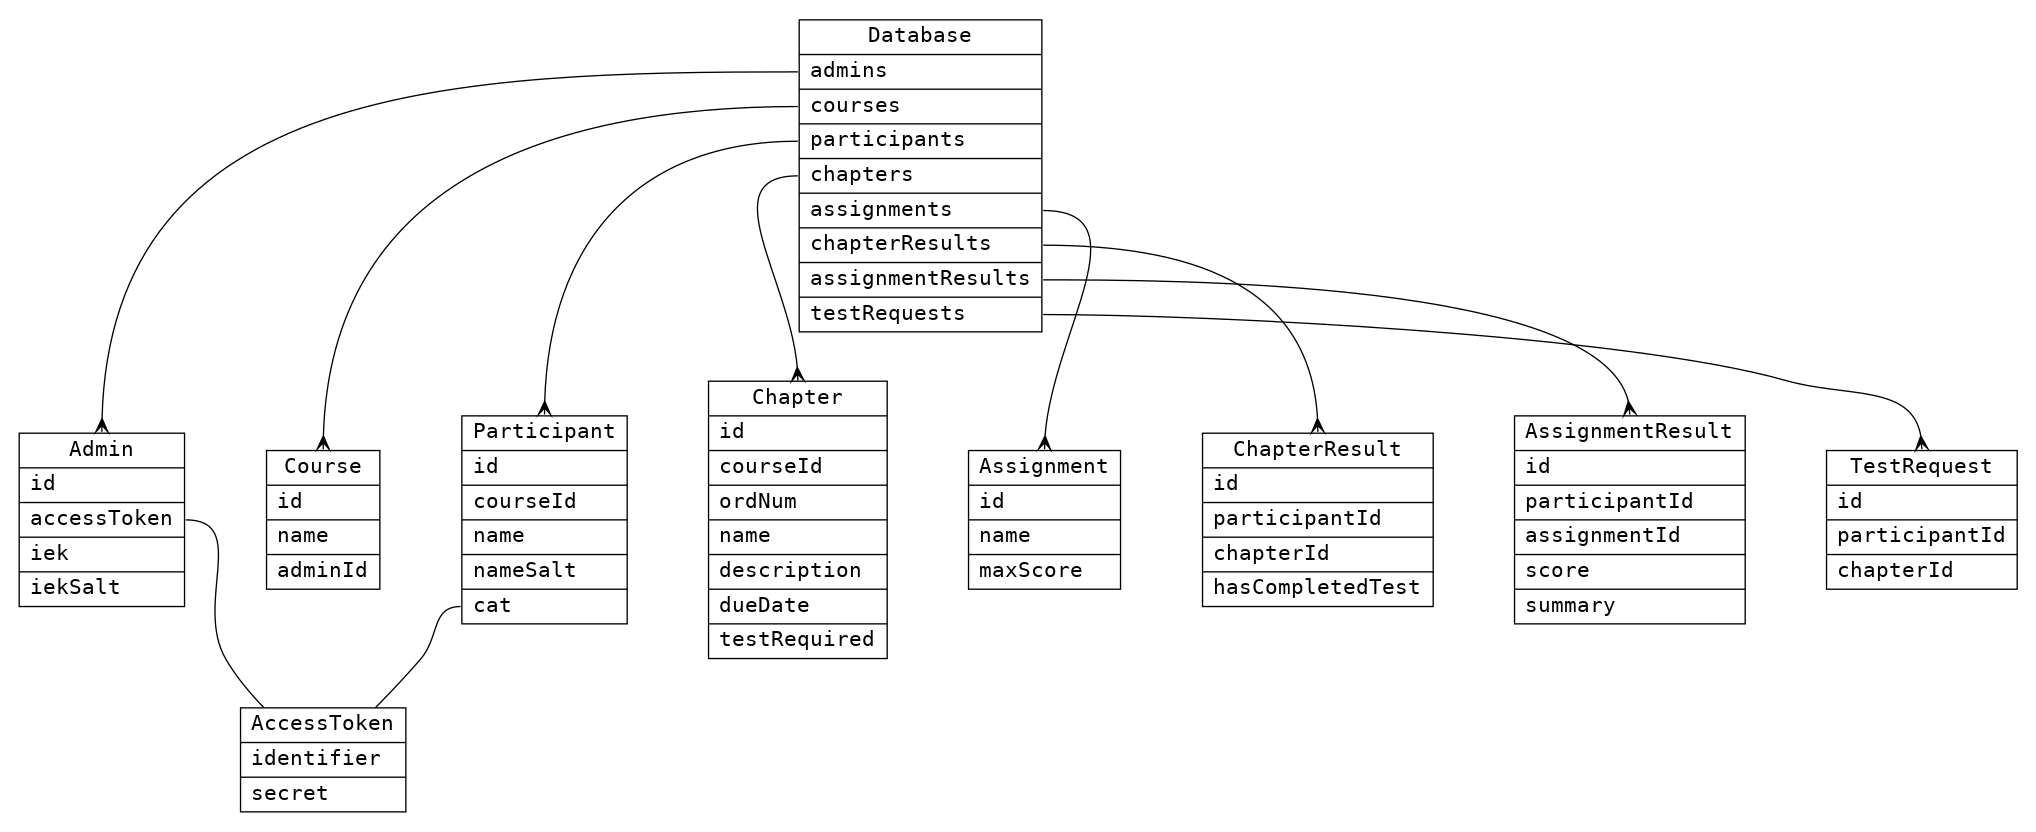
\includegraphics[angle=90,height=.85\paperheight]{easymark_data_model.png}
	}
\end{document}
